\resetgraphicspath
\appendtographicspath{{./Chapter 1/figures/} }
\appendtographicspath{{./Chapter 1/figures/Procedural/} }
\appendtographicspath{{./Chapter 1/islands/} }
\appendtographicspath{{./Chapter 1/Results/} }
\appendtographicspath{{./Chapter 1/Results/Procedural/} }
\appendtographicspath{{./Chapter 1/Results/Reproduction/} }
\appendtographicspath{{./Chapter 1/Results/results_cGAN_PG25/} {./Chapter 1/Results/results_cGAN_PG25/Renders} }
\appendtographicspath{{./Chapter 1/Results/volcanic/} }
\appendtographicspath{{./Chapter 1/figures/Smoothmax/} }
\appendtographicspath{{./Chapter 1/figures/vector_field/} }
\appendtographicspath{{./Chapter 1/figures/SOTA/coral theories/} }
\appendtographicspath{{./Chapter 1/figures/SOTA/sketching/} }

\chapter{Automatic generation of coral reef islands}
\label{chap:coral-island}
\teaser{
    \autofitgraphics[]{Teaser1.png, Teaser2.png, Teaser3.png}
    \caption[Example of an island with gradual subsidence]{Given a free hand-drawn sketch of the different regions of an island (bottom inset of each example), our method generates a corresponding height field using neural networks. Subsidence (gradual sinking of land) is controlled by the user in the luminosity channel of the input. These examples show the gradual subsidence of the same island over time.}
    \label{fig:teaser_cGAN}
}

\abstract
In this chapter, we propose a procedural method for generating single volcanic islands with coral reefs based on user sketches from two projections commonly used in geological and remote sensing domains: a top view defining the island's shape, and a profile view, establishing its elevation. 
We add a user-defined wind field that deforms the island to mimic long-term effect of wind and wave, providing finer user control over the island's shape.
Next, we model the coral growth on the island following biological observations.
This results in a terrain height field of the island and its surrounding reef. 
Our method creates a large variety of coral reef island models which we used to train a conditional Generative Adversarial Network (cGAN). 
By applying data augmentation, the cGAN enhances the variety in the generated islands, providing users with greater freedom and intuitive controls over the shape and structure of the final output.
\pagebreak

\minitoc

\section{Introduction}
\label{sec:coral-island-introduction}

\begin{figure}[H]
    \autofitgraphics[]{Kauai_island.png, Tuvuca_island.png, Mascarene_island.png, Cocos_island.png}
    \caption[Different islands with coral reefs]{Kauai Island, Tuvuca Island, Mascarene Island, and Cocos Island (from left to right) are islands formed through an identical geological process; however, their shapes vary greatly, from a full island with fringing coral reef (leftmost) to a complete atoll (rightmost).}
    \label{fig:coral-island-island-examples}
\end{figure}

The scarcity of high-resolution data, the need for volumetric and multi-scale representations, and the strong influence of biological and hydrodynamic processes present unique modelling challenges for underwater landscapes. Among these environments, coral reef islands are of particular interest and complexity. They result from a long-term interplay of volcanic activity, coral growth, erosion, and subsidence, producing highly distinctive morphologies that procedural techniques must capture if they are to generate convincing seascapes. 

We propose a simplified user-centered interface to focus on the overall large-scale modelling of coral reef islands using sketching methods to avoid tedious user control over a large range of ecological parameters.

To better understand these morphologies, we begin by recalling the classical geological explanation of their formation, as proposed by Charles Darwin in the 19th century \cite{Darwin1842}. His subsidence theory remains a foundational description of how volcanic islands gradually transform into barrier reefs and atolls (such as the islands presented in \cref{fig:coral-island-island-examples}), and it provides the conceptual backdrop for our generative model.

According to this theory, these islands begin as volcanic landmasses, created when magma from the Earth's mantle erupts through the ocean floor and builds up layers of volcanic rock, eventually rising above sea level (\cref{fig:coral-island-island-growth}). In tropical waters, these volcanic islands create ideal conditions for coral reefs to develop. Corals, thriving in the shallow, sunlit waters around the island, initially form fringing reefs attached to the island's coastline (Stage 1 in \cref{fig:coral-island-reef-growth}).

\begin{figure}
    \autofitgraphics{other_images/Drawings/Volcano-color.jpg}
    \caption[Volcanic island formation process]{Volcanic islands rise above hotspots. The rise of magma from the hotspot forms a seamount. Consecutive eruptions from the volcano grow the seamount until the peak emerges above sea level. The ground above and close to sea level is affected by hydraulic, aeolian, and coastal erosion.}
    \label{fig:coral-island-island-growth}
\end{figure}

As time passes, the volcanic island undergoes subsidence, a slow sinking process caused by the cooling and contraction of the Earth's crust beneath the island. In response, corals continue to grow upwards to remain within the photic zone, where sunlight supports their survival. This upward growth combined with subsidence leads to the formation of barrier reefs, that become separated from the island by a lagoon as it sinks further (Stage 2 in \cref{fig:coral-island-reef-growth}).

Eventually, the volcanic island may submerge completely, leaving only the coral structure visible above water. This process results in an atoll: a ring-shaped reef encircling a central lagoon (Stage 3 in \cref{fig:coral-island-reef-growth}). Over geological time, the island's shape evolves from a prominent volcanic peak into a coral-dominated reef system shaped by subsidence, coral growth, and erosion.

\begin{figure}
    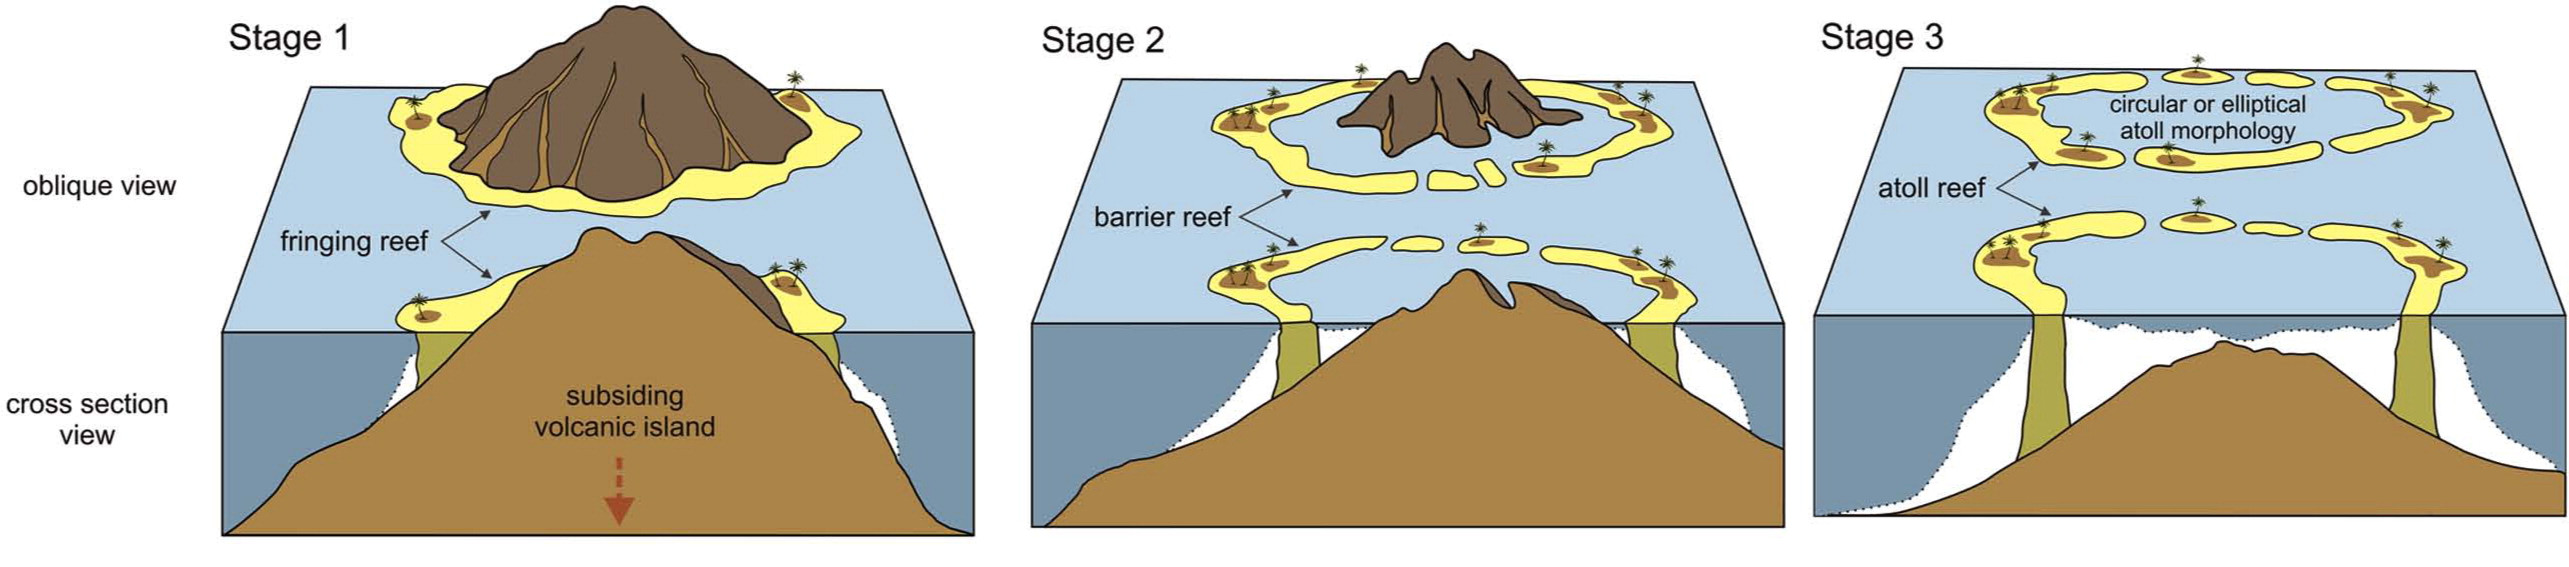
\includegraphics[width = \linewidth]{other_images/Drawings/Darwin_corals-color-Terry2012.jpg}
    \caption[Darwin's subsidence theory]{Coral colonies grow near sea level, forming a fringing reef (Stage 1). The island sinks slowly (subsidence); the coral reef continues its growth to keep living coral colonies in the photic zone. The sinking island increases the size of the lagoon, forming a barrier reef island (Stage 2). When the peak of the island is below the surface of the lagoon, an atoll is formed (Stage 3) \cite{Terry2013}.}
    \label{fig:coral-island-reef-growth}
\end{figure}

Simulating the formation of coral reef islands presents significant challenges due to the complex interplay of geological, environmental, and biological factors \cite{Hopley2014}. One major difficulty lies in capturing the long-term subsidence of volcanic islands, occuring over millions of years, and the concurrent upward growth of coral reefs that rely on environmental conditions (e.g., water depth, temperature, sunlight, ...). This combination of slow geological processes and dynamic biological growth is inherently challenging to replicate in a computational model.

Additionally, the biological aspects of coral growth are inherently dependant on environmental factors. Coral reefs grow only within a specific range of water depth and sunlight, and their growth patterns are influenced by reef ecosystem's health and resources availability. Accurately modelling these biological dependencies in a procedural system is challenging, as these factors are numerous and difficult to generalise. Moreover, the scarcity of data available obstructs global understanding of these biomes. In a recent high-resolution mapping of shallow coral reefs \cite{Lyons2024}, researchers estimated the total surface area of this biome to cover less than 0.7\% of Earth's area, and more specifically that coral habitat represents less than 0.2\%.

Existing terrain generation methods, such as Perlin noise-based algorithms or uplift-erosion models, are often ill-suited for these multi-disciplinary processes. Although they generate natural-looking landscapes (such as alpine landscapes, representing about a quarter of land area \cite{Korner2014}), they do not account for the unique geological and biological interactions critical for coral reef island development, resulting in a lack of coherence. Capturing these dynamics, while also providing user control during the modelling of a terrain, requires a balance between realism and procedural flexibility, allowing for both accurate computationally expensive simulation of natural processes and intuitive user control in interactive time.

The formation of these islands involves processes at multiple scales, from the growth patterns of coral colonies to large-scale sediment transport, which are difficult to simulate directly. As a result, purely procedural or physics-based simulations fail to produce convincing or diverse coral reef island landscapes. On the other hand, deep learning methods are inoperable due to the extremely small amount of data, and the scarcity of high-resolution DEMs of these regions.

Despite advances in terrain generation, current methods struggle to support user-controlled design of specific island shapes and achieving realism without real data. Coral reef islands exemplify this gap: we lack datasets to directly train deep learning models, and purely procedural methods require expert tuning to mimic their features.

To address these challenges, we use procedural generation as an initial step in our global pipeline. In this step we employ algorithmic rules to synthesise terrain features, allowing us to encode basic patterns of coral reef island formation. However, such algorithms are inherently rigid: they are tailored to a narrow family of shapes (in our case, radially organised and centred islands) and often rely on mathematical controls that are unintuitive for non-expert users. In our work, we use a procedural model not as the final solution, but as a means to efficiently create a large and diverse set of training examples for a learning-based model. Specifically, by adjusting procedural parameters, the procedural pipeline produces varied island scenarios. Each synthetic example is represented by a detailed terrain height field and a corresponding semantic label map that marks different regions, providing structured input-output pairs for the learning stage.

We then train and deploy a conditional Generative Adversarial Network (cGAN) as the core of our method. A cGAN is a type of deep learning model that learns to generate realistic data based on an input condition or context. In our case, the cGAN takes as input the semantic label map of an island (a label layout indicating regions such as ocean, reef, beach, and mountain) generated by the procedural step and learns to produce a plausible island height field that matches this layout. By training on a large set of examples from the procedural generator, the cGAN captures subtle terrain features and variations unique to coral reef islands, going beyond what hard-coded procedural rules can achieve thanks to the application of data augmentation.

Once the cGAN is trained on a sufficiently large and varied set of synthetic islands, it is used on its own to generate new island terrains. At this stage, our procedural generation module, only necessary to provide training data, is not required for creating new islands. Instead, a user provides a semantic map using digital drawing or another simple algorithm, and the cGAN generates a plausible island terrain accordingly. To summarise, our pipeline leverages procedural modelling to create a training dataset, and then relies on the learned cGAN model for the final generation of coral reef islands. In this way, we overcome the scarcity of real data by procedurally generating training examples, and overcome the rigidity of procedural rules through cGAN-based learning.


The key contributions of this chapter are:
\begin{Itemize}
    \Item{} a novel sketch-based procedural algorithm for shaping island terrains from top and profile views,
    \Item{} the use of a deep learning model trained on synthetic data derived from procedural rules, acting as an abstraction layer that hides underlying complexity,
    \Item{} a demonstration that the cGAN approach tolerates imprecise, low-detail user input sketches, broadening usability, without the need for cutting-edge network architectures,
    \Item{} and an insight that procedural generation remains essential to produce training data in data-sparse domains, illustrated by the example of coral reef islands.
\end{Itemize}
These contributions collectively show a pathway for blending user-driven design with learning-based generation for terrain modelling.

\section{State of the art}
\label{sec:coral-island-SotA}

Procedural terrain generation and sketch-based modelling have each seen significant advances over the past decades, yet neither alone fully addresses the particular challenges of coral reef island synthesis. On the one hand, classic noise-based and physically driven methods (Perlin noise, hydraulic erosion, uplift-erosion models) excel at producing broad, natural-looking landscapes but lack the biologically inspired reef geometries and dynamic island evolution governed by subsidence and coral growth. On the other hand, sketch-based tools give users intuitive control over silhouettes and terrain profiles, but typically require expert parameter tuning to achieve realism and do not model long-term geological or ecological processes. More recently, deep learning, especially GANs and cGANs, has emerged as a powerful way to learn terrain features and geological rules from data, yet it relies on large, labelled datasets that are scarce for coral reef islands. 

In this section, we first review the key geological theories that explain reef formation, then examine traditional procedural terrain generators, followed by an overview of sketch-based terrain editing frameworks, and finally discuss recent advances in GAN-based terrain synthesis.

\subsection{Coral reef island formation theories}
\label{sec:coral-island-sota-coral-theories}

Since Darwin first proposed his subsidence theory, presented in \cref{sec:coral-island-introduction}, geologists and biologists have debated how exactly coral reefs have formed around land masses. In this section we present three major alternatives to Darwin's theory, before explaining why Darwin's unified subsidence model provides the most direct foundation for our procedural generation.

\begin{Itemize}
    \AltTextImageBottom{
        \Item{} \textbf{Murray's stand-still theory \cite{Murray1880}} \\
        Murray argued that reefs could develop on stable, non-sinking platforms, with coral growth keeping pace with modest sea-level changes rather than underlying land subsidence. He proposed that as long as water depth remained within the photic zone, reefs would accrete upward solely in response to environmental sea-level fluctuations, and continuously seaward, forming a gradual structure from a fringing reef to barrier reef (\cref{fig:coral-island-murray-theory}). Atolls in this theory are mainly created by the degradation of the middle island through aeolian and coastal erosion until it becomes completely submeged. Murray's emphasis on environmental stability and gradual sea-level change was supported by early observations of island terraces and reef growth patterns. However, later drilling and seismic data revealed volcanic foundations buried beneath reef limestones on many atolls, which are evidence of true subsidence that Murray's theory cannot explain.
    }{Murray.pdf}% }{Murray-drawing1.png, Murray-drawing2.png, Murray-drawing3.png}
    {In Murray's theory, with the island fixed in place but reducing in size due to erosion, reefs (red) simply remains at sea level and grows outwards (producing fringing reefs, then barrier reefs, and eventually atolls) without any subsidence, leaving only the inside reef filled with sand (yellow) forming a lagoon.}{fig:coral-island-murray-theory}{Murray's stand-still theory}

    \AltTextImageBottom{
        \Item{} \textbf{Daly's glacial-control theory \cite{Daly1915}} \\  
        Daly shifts the focus from steady subsidence to global sea-level oscillations driven by glacial-interglacial cycles. He argues that reefs thrive during high sea levels in interglacials but are exposed and eroded during glacial lowstands. As sea levels rise again, the wave-cut benches left behind provide ideal habitats for new coral colonies, which grow upward with the water level and can develop into barrier reefs or atolls once sea level overtops the island (\cref{fig:coral-island-daly-theory}). He supports this model by pointing to multiple reef terraces at different elevations and well-documented 100m sea-level drops during ice ages as support for this cycle-driven reef development. The plausibility of Daly's model lies in its direct link with climatic data and the clear geomorphic signatures of past sea-level stands. Yet, core samples often show uninterrupted reef accretion atop subsiding volcanic bases, indicating that glacial cycles alone cannot account for continuous reef "keep-up" growth.
    }{Daly.pdf} % }{Daly-drawing1.png, Daly-drawing2.png, Daly-drawing3.png}
    {In Daly's theory, repeated sea-level drops expose the reef to wave planation and erosion into a flat bench (grey), and subsequent high stands see new coral rims (red) accrete on that outer terrace to form a lagoon-separated barrier reef.}{fig:coral-island-daly-theory}{Daly's glacial-control theory}

    \AltTextImageBottom{
        \Item{} \textbf{Droxler's karstification theory \cite{Droxler2021}} \\  
        In contrast to models based on volcanic subsidence, Droxler et Jorry attribute atoll formation to repeated karst dissolution of a broad carbonate platform during low-sea-level glacials, followed by renewed coral accretion in interglacials (\cref{fig:coral-island-droxler-theory}). High-resolution bathymetry and drill cores reveal karst-etched depressions beneath certain atoll crests, supporting this cyclic exposure-dissolution mechanism. While compelling for extensive carbonate shelves, this theory hinges on pre-existing flat platforms and meteoric water circulation (water originating from precipitation), which are conditions uncommon on volcanic seamounts. As a result, Droxler's model explains atoll rings on continental carbonate foundations but does not readily apply to volcanic island reef systems. 
    }{Droxler.pdf} % }{Droxler_placeholder.png}
    {A broad carbonate platform (grey) is exposed and karstified during low-sea-level glacials, then drowns and is rimmed by reef growth (red) at its outer edge during high stands, yielding an atoll-style rings.}{fig:coral-island-droxler-theory}{Droxler's karstification theory}

\end{Itemize}

Of all the competing hypotheses, Charles Darwin's subsidence model offers several compelling advantages for our procedural island generation due to its simplicity, historical significance, and effectiveness \cite{Tomascik1997}. This theory provides a straightforward framework outlining a clear progression from fringing reefs to barrier reefs to atolls as a volcanic island subsides, which can be easily modelled, making it practical for generating plausible island landscapes. This simplicity not only ensures predictability in simulation outcomes but also reduces computational demands, which is particularly beneficial for interactive edition applications. Additionally, Darwin's model provides a foundational basis upon which more complex phenomena (sea-level changes and climatic effects), considered as secondary factors in the geological formation of islands, could be layered. This allows us to start with a basic model and, in the future, add complexity as needed, offering flexibility in simulation design.

In our approach, we translate the core principles of Darwin's theory into a procedural generation model, emulating the gradual sinking of volcanic islands while coral reefs grow to keep pace with changing sea levels. This allows us to realistically model the progressive transformation of islands from volcanic landmasses to coral-dominated atolls. By capturing this interplay, we procedurally generate a wide variety of island structures that reflect real-world geological processes.

In generating synthetic coral reef islands, we adopt a set of simplifying assumptions that are interpreted by the formation process from Darwin's theory and field observations:
\begin{Itemize}
    \AltTextImage{
        \Item{} \textbf{Radial symmetry and radial arrangement of features} \\
        While volcanic islands do not have a perfect circular shape and reefs are not exact rings, they grow outward in roughly concentric belts (looking at the island in \cref{fig:coral-island-radial-symmetry-assumption}, we see the typical layout mountain-beach-lagoon-reef-ocean). Anchoring our sketch-to-terrain engine on this radially organised structure offers two main benefits to the user: a single intuitive control over the overall island shape and while keeping distance computations simple and efficient.

        \Item{} \textbf{Uniform profile shape} \\
        Although real islands have ridges, valleys, local bumps and many other features, we simplify the model to a single elevation curve from centre to edge, making the profile-view sketch a one-dimensional drawing, enabling users to modify elevation with a single stroke.
    }
    {Tuvuca_island.png}{Aerial view of Tuvuca Island, Lau Archipelago, Fiji.}{fig:coral-island-radial-symmetry-assumption}{Aerial view of Tuvuca Island}

    \AltTextImage{
        \Item{} \textbf{Subsidence and coral "keep up" growth} \\
        Actual reefs respond to light, nutrients, and biology, but the dominant effect is that corals grow vertically to stay near the photic zone. We decouple coral growth from subsidence and simply keep reef heights in a fixed band beneath the surface, capturing Darwin's core insight using minimal parameters.

        \Item{} \textbf{Wind and wave deformation} \\
        To represent coastal erosion resulting from sediment transport and complex hydrodynamics \cite{Terry2013}, we simplify the model by using a vector field painted by the user representing wind and wave directions, deforming the global island (\cref{fig:coral-island-wind-deformation-assumption} suggest that island outlines are influenced by the average wind direction). This vector field allows radial symmetry to be broken in a controllable way, without relying on a full erosion simulator.
    }
    {Mauritius_wind.png}{Mauritius is deformed. We see a deep slope on the west side while the east side has a gentle slope. The wind rose, showing in which direction the mean wind velocity is pointing, is correlated with this deformation.}{fig:coral-island-wind-deformation-assumption}{Mauritus Island and average wind direction}

    \Item{} \textbf{Independence of islands} \\
    While archipelagos share currents, sediments, and flood each other's lagoons, simulating multi-island interactions is computationally expensive and hard to control. We treat each island as an isolated entity to generate multi-island scenes by using a simple blending of individual islands, keeping our method fast and predictable.

\end{Itemize}

\midConclusion

These assumptions, grounded in theories of coral reef island formation, provide a practical foundation for procedural modelling. While they simplify the full complexity of geological and biological processes, they capture the essential dynamics needed to produce plausible island structures. Simultaneously, they ensure our system remains intuitive, controllable, and computationally efficient, enabling the generation of diverse and plausible islands suitable for interactive design.





\subsection{Traditional terrain generation methods}
\label{sec:coral-island-sota-traditional}

Procedural generation of terrain has been a well-researched area in computer graphics and simulations, where the goal is to create large, realistic landscapes with minimal manual input. Various methods have been developed over the years to generate terrains automatically, from noise-based methods to physically based erosion simulations, sketch-driven mechanisms, and more recently, deep learning techniques.

However, coral reef islands present unique challenges due to the combination of long-term geological processes (mainly subsidence and coral reef growth) and environmental interactions (i.e. erosion caused by wind and waves). In this section, we review the key techniques proposed for terrain generation, highlighting their limitations for coral reef island formation, and positioning our work as an approach that addresses these challenges.

\subsubsection{Noise-based terrain generation}

\begin{figure}
    
\includegraphics[width = \linewidth]{noise_examples3.pdf}
    \caption[Islands generation using fBm noise and falloff masks]{Three different results of an island generated from noise functions. In each case, the initial height field is identical, computed using flow noise. The falloff masks are created by combining fBm noise, modulated by the Euclidean distance from the image centre, and further shaped through domain warping and power-law remapping of the mask values. The only parameter modified between the three examples is the exponent used in this remapping. The resulting islands differ significantly in shape and scale, and the method offers limited control over specific coastal features such as lagoons and reefs.}
    \label{fig:coral-island-noise-example}
\end{figure}

Noise-based procedural generation remains one of the most widely used techniques for creating natural-looking terrains on height fields. Perlin noise \cite{Perlin1985}, Simplex noise \cite{Perlin2001}, and the Diamond-square algorithm \cite{Fournier1982} are foundational algorithms that generate pseudo-random yet continuous variations across a grid, producing terrain features that resemble organic landscapes. These techniques have been widely adopted in computer graphics and game development due to their efficiency and visual appeal.

Beyond basic noise functions, advanced techniques such as fractal Brownian motion (fBm) and multifractal noise have been introduced to add finer-scale variation and detail \cite{Musgrave1989,Ebert2003}. fBm combines multiple layers, or "octaves," of noise at different frequencies and amplitudes, producing terrains that exhibit realistic and varied features. The combination of noise with domain warping and signal processing techniques has been explored in depth in procedural modelling literature \cite{Reinhard2010}, enabling further control over visual complexity and terrain realism.

Noise functions are often paired with falloff maps to produce island-like terrains, where elevation gradually decreases towards the edges of the domain, mimicking coastlines and basic island shapes (see \cref{fig:coral-island-noise-example}). Various methods for enhancing island generation using noise and falloff blending have been proposed for applications in games and virtual worlds \cite{Olsen2004}. While these techniques excel at producing large, visually diverse landscapes quickly, they suffer from several key limitations when applied to the modelling of coral reef islands.

However, limitations arise when applying these methods to coral reef islands as noise-based modelling lack grounding in geological or biological reality. They generate spatial patterns through mathematical noise, not through simulations of real-world processes such as volcanic subsidence or coral accretion. The signal processing parameters typically involved (frequency, lacunarity, gain, amplitude, ...) are tuned for visual effect rather than scientific plausibility. As highlighted in procedural modelling surveys \cite{Smelik2009,Galin2019}, this disconnect results in a lack of semantic control and poor correlation with actual environmental dynamics, making it difficult to represent phenomena such as reef rings, lagoons, or atoll structures in a biologically or geologically coherent way.

Moreover, the biological aspects of coral growth are inherently tied to environmental conditions. Coral reefs form and persist only within specific ranges of water depth, sunlight, salinity, and water quality. Their growth patterns are further influenced by ecological health, nutrient availability, and symbiotic relationships. These dependencies are extremely difficult to capture in procedural noise models, which are not designed to reproduce such complex and coupled dynamics.

Our approach goes beyond the randomness of noise-based generation by incorporating real-world geological and biological processes into the terrain formation pipeline. Specifically, we model the gradual subsidence of volcanic islands and the upward growth of coral reefs, both of which are central to the long-term evolution of coral reef islands. By embedding these natural processes directly into the generation algorithm, we produce terrains that are not only more realistic but also more controllable. This integration of scientific modelling with procedural flexibility allows us to overcome the inherent limitations of traditional noise-based techniques and more accurately represent the complex formation of coral reef island systems.

\subsubsection{Simulation-based modelling}

Simulation-based terrain modelling methods aim to increase realism by replicating natural processes such as erosion, sediment transport, tectonic uplift, and vegetation growth. Unlike noise-based strategies, which rely on random functions, simulation-based processes model causality and temporal dynamics to describe how a terrain evolves over time under physical or biological forces. These methods are often used to enhance base terrains, adding geologically plausible detail and structure \cite{Benes2006, Smelik2009}.

\subsubsubsection{Hydraulic and thermal erosion}

Hydraulic erosion models simulate the impact of flowing water on the landscape by modelling erosion, sediment pickup, transport, and deposition. Early implementations by \cite{Musgrave1989} laid the groundwork for erosion in procedural generation, while more recent works have accelerated these simulations using GPU architectures \cite{Mei2007} and particle-based methods \cite{Neidhold2005}. These simulations either follow Eulerian fluid models or Lagrangian particle systems to capture terrain displacement.

Thermal erosion, by contrast, simulates mass movement due to gravity, redistributing material from steeper slopes to gentler gradients, akin to landslides or soil creep \cite{Benes2006}. These erosion models generate realistic fluvial networks and landforms, but they are parameter-sensitive and computationally expensive.

Moreover, such models are generally designed for terrestrial landscapes and lack mechanisms for simulating underwater sedimentation, reef growth, or biogenic processes crucial to coral reef island formation. These models typically simulate time scales relevant to geomorphological processes (hundreds to thousands of years), which are mismatched with both the faster dynamics of biological processes (e.g., coral growth) and the slower geological evolution of reef islands.

We propose our new particle-based erosion simulation method, adapted for underwater and terrestrial landscapes, in \cref{chap:erosion}.

\subsubsubsection{Tectonic uplift and geologic simulation}

Geological simulation approaches such as those proposed by \cite{Cordonnier2016, Cordonnier2017a} and extended by \cite{Schott2023} model terrain evolution through crustal deformation and tectonic uplift. These methods simulate isostatic adjustments, plate tectonics, or local uplift phenomena, often over geological timescales.

Although well-suited for mountain-building processes or fault line modelling, these methods are not designed to account for biogenic terrain formation, such as coral reef accretion, which is critical for simulating coral reef islands. As a result, despite being physically grounded models, they do not capture the coupled geological and biological dynamics necessary for representing the long-term evolution of reef islands.

\subsubsubsection{Vegetation and ecosystem dynamics}

A number of simulation-based terrain models integrate ecological dynamics to reflect the feedback between terrain and living systems. For instance, \cite{Ecormier-Nocca2021} and \cite{Cordonnier2017b} simulate interactions between vegetation and terrain erosion, modelling plant colonisation, growth, and their influence on soil stability and moisture retention.

These ecosystem simulations allow more complex landscape evolution by considering biotic agents; however, they are designed primarily for terrestrial plants and temperate ecosystems. Coral colonies, in contrast, are marine organisms with strict environmental requirements (e.g., limited depth, adequate sunlight, nutrients presence, warm water temperatures, ...). Accurately simulating these dependencies would require significant computational resources. We present a deeper analysis of current ecosystem simulations in \cref{chap:semantic-representation}'s state of the art.

Furthermore, coral growth is not a passive process such as sediment accumulation, but an active accretion system that builds calcium carbonate structures over thousands of years. These unique growth mechanisms, constrained by marine ecology, fall outside the scope of existing vegetation or soil-plant-water feedback models.

\citeName{Li2021} propose to procedurally synthesizes coral colonies structures by emulating stochastic reef growth with a Diffusion-Limited Aggregation process, producing reef patterns but does not propose control over the simulation \cite{Li2021}. The integration of user input such as sketch interfaces remains essential for controlling the generated output.

\midConclusion

While simulation-based models represent a significant advancement over purely procedural models, they fall short in capturing the coupled geological and biological dynamics that shape coral reef islands. They are either computationally intensive, domain-specific, or biologically inapplicable, highlighting the need for a new class of terrain generation tools that embed long-term marine biogeomorphological processes into the procedural pipeline.


\subsection{Sketch-based terrain modelling}
\label{sec:coral-island-sota-sketches}

The term "sketching" encompasses several definitions: either refering to performing hand or body gestures, creating a rough drawing, or outlining an idea in a simplified form. Accordingly, sketch-based modelling in 3D computer graphics can be understood through three complementary perspectives, each centred around a distinct core concept: interaction, construction and interpretation.

First, "sketching" may focus on interaction, where gestures captured through hand or body motion are used to manipulate virtual objects, often in immersive environments (virtual or augmented reality), using established techniques such as sculpting and distortion \cite{Olsen2009, Cook2009}. Second, "sketching" may involve construction, where simple geometric primitives (curves, parametric shapes, implicit surfaces, ...) are combined under constraints to build a more complex model. Finally, "sketching" may centre on interpretation, where the user draws strokes on a 2D canvas and the system analyses their meaning to generate a plausible 3D model.

While sketch-based modelling encompasses a wide range of techniques, including gesture-driven interaction in immersive environments, this work focuses primarily on construction and interpretation aspects. In particular, construction serves as the foundation for procedural generation techniques using geometric primitives and constraints, while interpretation becomes relevant when exploring data-driven approaches using deep learning to infer terrain structure from sketches. Interaction-based techniques, though significant in other contexts, fall outside the scope of this work.

To clarify terminology in this chapter, we refer to the constructive approach as sketch-based, and to the interpretive, learning-driven approach as learning-based. It is important to note, however, that the boundaries between these categories are inherently blurry and often overlap in practice.

In procedural terrain generation, sketch-based construction workflows enable users to shape landscapes by manipulating high-level geometric primitives through intuitive sketching interfaces. These methods allow the definition of key terrain features (mountains, valleys, coastlines, ...) by drawing their outlines on a two-dimensional canvas, which are then procedurally transformed into 2.5D or 3D terrain representations. This technique offers a high degree of control, making it particularly effective for creative applications such as video games and robotics simulations, where modelling is primarily user-driven.

\subsubsection{Curve-based modelling}

Sketch-based terrain generation often begins with user-defined curves which act as high-level constraints to guide the shape of the terrain. These curves represent silhouettes, ridgelines, valleys, or feature outlines. Once defined, they are interpreted by the system and translated into elevation changes through various computational techniques. This type of approach allows for intuitive control over large-scale landforms while maintaining a procedural foundation for terrain synthesis.

\AltTextImage{
    One of the earliest and most influential works in this domain was introduced by \citeName{Gain2009} (\cref{fig:coral-island-Gain2009}), enabling users to sketch silhouettes, ridges, and spine curves to define complex terrain structures \cite{Gain2009}. The method employs multiresolution surface deformation and propagates wavelet-based noise from the sketched features to their surroundings, allowing users to generate detailed, natural-looking terrains from minimal input. This method demonstrated the effectiveness of combining intuitive sketch input with procedural detail synthesis.

    We draw direct inspiration from this work's dual-view sketching strategy, combining top-view and profile sketches, which closely aligns with our concentric curve and height-profile input approach.
}{sketchingGain2009-s.png}{\citeName{Gain2009} propose to edit terrains through sketching by diffusing a noisy height function over a bounded region (left), effectively modelling mountain ranges (right) \cite{Gain2009}.}{fig:coral-island-Gain2009}{\cite{Gain2009}'s sketching method}

\AltTextImage{
    Building on this idea, \citeName{Hnaidi2010} proposed a technique based on diffusion equations \cite{Hnaidi2010}. In their method, curves are annotated with geometric constraints (elevation, slope, and roughness), and a diffusion process is used to interpolate these constraints across the terrain surface. This results in smooth, continuous elevation fields that conform to user-defined features such as rivers, ridgelines, or cliffs (\cref{fig:coral-island-Hnaidi2010}). The use of parameterised curves as terrain anchors allows for precise control over landform shaping, while maintaining a high degree of automation.
}{sketching-Hnaidi2010.png}{\citeName{Hnaidi2010} define the surface by elevation curves with constrained slopes, forming with ease river beds and cliffs \cite{Hnaidi2010}.}{fig:coral-island-Hnaidi2010}{\cite{Hnaidi2010}'s sketching method}

\AltTextImage{
    In a different interaction paradigm, \citeName{Tasse2014} introduced a first-person sketching interface, where users draw terrain silhouettes from a particular camera viewpoint \cite{Tasse2014}. These silhouettes are then projected into 3D, and a deformation algorithm adjusts the terrain so that the drawn features are visible exactly as intended from the user's perspective (\cref{fig:coral-island-Tasse2014}). This method supports complex silhouettes with occlusions, T-junctions, and cusps, and represents an immersive and perceptually grounded approach to sketch-based terrain editing.
}{sketchingTasse2014-s.png}{\citeName{Tasse2014} use sketching in association with camera position and direction to constrain the edition of height fields \cite{Tasse2014}.}{fig:coral-island-Tasse2014}{\cite{Tasse2014}'s sketching method}

\smallConclusion

These methods demonstrate the expressive power of curves as terrain-defining elements. By enabling users to sketch intuitive shapes and constraints, they bridge the gap between artistic intent and procedural complexity. Curve-driven methods remain foundational in terrain modelling, particularly when user control over large-scale structure is essential. While we do not use the diffusion model, the idea of sketch-defined elevation constraints along curves informs our use of user-defined shape boundaries.

\subsubsection{Constraint-based modelling}

Constraint-based and gradient-based families of methods focus on exerting precise control over terrain features via formal specifications such as elevation values, slopes, or gradient fields. These methods prioritise structural accuracy and procedural consistency, making them particularly suited to applications that demand terrain realism, integration with geographic data, or fine-grained editing capabilities.

\AltTextImage{
    A representative example of constraint-based modelling is presented by \citeName{Gasch2020}, proposing a method for procedural terrain generation that respects user-defined elevation constraints \cite{Gasch2020}. Their system allows users to fix values at specific control points (e.g., paths, landmarks) and then solve a system of equations to propagate these constraints throughout the terrain. The method integrates these constraints with a noise-based procedural function to preserve natural randomness while conforming to user intent (\cref{fig:coral-island-Gasch2020}). This approach is especially valuable when generating terrains that must align with real-world data or gameplay constraints.

    We do not adopt this constraint-solving mechanism, but conceptually relate our profile sketch input to a localised height constraint.

}{sketching-Gasch2020-s.png}{\citeName{Gasch2020} use a top-view sketch to apply constraints (a) on the noise function modelling a terrain, creating an intuitive means to create paths and roads in the resulting terrain (b and c) \cite{Gasch2020}.}{fig:coral-island-Gasch2020}{\cite{Gasch2020}'s sketching method}

\AltTextImage{
    Extending this idea, \citeName{Talgorn2018} introduce a real-time sketch-based terrain generation system based on a GPU-accelerated implementation of midpoint displacement \cite{Talgorn2018}. Users sketch curves with explicit elevation values, which act as absolute constraints, and the system extrapolates and interpolates terrain surfaces in real-time. Moreover, the user input influences the elevation constraint and interpolation method properties of the midpoint displacement algorithm using the Red, Green and Blue channels (\cref{fig:coral-island-Talgorn2018}). Their model supports both global and local control over interpolation curvature and roughness, and introduces semantic labelling of sketched features (e.g., ridges vs. rivers) to influence how terrain propagates around constraints. This combination of sketch-based input, constraint propagation, and semantic control enables expressive, large-scale terrain modelling at interactive speeds. We adopt their notion of semantic labels and hierarchical constraint propagation to support real-time terrain shaping with sketch-defined features without the fractal interpolation.
}{sketching-Talgorn2018.png}{\citeName{Talgorn2018} use top-view sketching to encode properties in the noise function used to model the terrain surface \cite{Talgorn2018}.}{fig:coral-island-Talgorn2018}{\cite{Talgorn2018}'s sketching method}

\AltTextImage{
    Building on the need for more intuitive editing, \citeName{Guerin2022} introduce gradient domain paradigm for terrain modelling \cite{Guerin2022}. Rather than specifying elevation values directly, users interact with slope-based representations, allowing for the manipulation of terrain inclination and the integration of local edits into global terrain structure (\cref{fig:coral-island-Guerin2022}). By controlling terrain gradients and reconstructing elevation through integration, this method enables seamless blending between regions and supports a natural editing workflow, particularly for sculpting realistic mountain ridges, valleys, or plateaus.
    This gradient-domain editing paradigm offers interesting insights; we adopt an alternative approach as we operate in the elevation domain with semantic control.
}{sketching-Guerin2022.png}{\citeName{Guerin2022} apply gradient (left) and height (right) constraints on curves and diffuse them on the terrain to create landscapes with lightweight and multi-scale representations \cite{Guerin2022}.}{fig:coral-island-Guerin2022}{\cite{Guerin2022}'s gradient domain terrain modelling}

\smallConclusion

Both paradigms offer complementary strengths: constraint-based methods ensure precise adherence to user-defined features or data sources, while gradient-based systems provide fluid, perceptual control over terrain shaping. Together, they represent a shift toward high-level modelling tools that maintain procedural expressiveness while granting users a deeper degree of terrain control.

\subsubsection{Semantic terrain representation}

Beyond geometric sketching and low-level constraints, a third class of methods explores high-level terrain construction, where users guide terrain generation using abstract or semantic inputs. These approaches aim to simplify the authoring process by allowing users to describe what a terrain should contain (e.g., a mountain or a valley) without specifying how to generate its geomety. Such methods often rely on symbolic sketching, sparse representations, or domain-specific visual cues, offering powerful tools for conceptual design and inverse procedural modelling.

\AltTextImage{
    In this vein, \citeName{Genevaux2015} propose a method for representing terrains as sparse combinations of procedural primitives, referred to as "terrain atoms" \cite{Genevaux2015}. These atoms are stored in a dictionary and are either extracted from real-world data or generated synthetically. The terrain is modelled as a linear combination of these features, forming a Sparse Construction Tree that blends primitives in a compact and expressive form (\cref{fig:coral-island-Genevaux2015}). This representation facilitates terrain editing, amplification, and reconstruction from coarse user input.
}{sketching-Genevaux2015-1.png,sketching-Genevaux2015-2.png}{\citeName{Genevaux2015} symbolically define a terrain by an aggregation of patches with real-world meaning \cite{Genevaux2015}.}{fig:coral-island-Genevaux2015}{\cite{Genevaux2015} sparse terrain representation}

\AltTextImage{
    An illustrative and domain-specific use case is presented by \citeName{Natali2012}, who introduce a system for rapid visualisation of geological concepts \cite{Natali2012}. Here, users sketch schematic representations of subsurface structures such as faults, folds, or strata, and the system generates plausible 3D visualisations of geological terrains (\cref{fig:coral-island-Natali2012}). Their tool is designed primarily for educational and exploratory purposes, enabling geoscientists and students to create, manipulate, and communicate complex geological scenarios through intuitive sketch input. Although it extends beyond traditional terrain elevation modelling, the work exemplifies how sketch-based systems can operate on a conceptual level and support domain-specific semantics.
    This work inspired our use of sketch strokes to define deformation fields, although our implementation targets structured terrain generation rather than schematic visualisation.
}{sketching-Natali-2012-original.png}{\citeName{Natali2012} use sketching to describe geological phenomena: (top) geological layer deformation, (middle) abrupt displacement from faulting, and (bottom) texture deformation \cite{Natali2012}.}{fig:coral-island-Natali2012}{\cite{Natali2012}'s geological storytelling method}

These high-level approaches demonstrate the potential of sketch-based modelling not only as a geometric tool, but as a semantic interface between human intention and terrain synthesis. By abstracting terrain construction into symbolic or feature-based representations, they allow users to create rich, expressive landscapes without directly engaging with low-level geometry, making them particularly valuable for tasks involving conceptual design, education, and inverse procedural modelling.

\midConclusion

The methods presented in this section illustrate the diversity of sketch-based approaches for constructive terrain modelling, from curve-driven shape control to constraint-based editing and semantic abstractions. While these methods offer valuable tools for intuitive user interaction and procedural shaping, they often lack ecological grounding, multi-view integration, or the ability to produce structured data suitable for training generative models. In our work, we reinterpret and adapt elements from these approaches (dual-view sketching, curve-based region definition, and deformation fields) to support the generation of coral reef islands through a hybrid procedural and learning-based pipeline. This constructive sketch-based foundation enables us to balance user control with scalable terrain generation in data-sparse domains.

\subsection{Deep learning}
\label{sec:coral-island-sota-deep-learning}

\begin{figure}
    
\includegraphics{schemaGAN_cGAN.jpg}
    \caption[GAN and cGAN architectures]{The general structure of GAN and cGAN networks is similar: (a) a generator network $G$ is trained to take some noise $z$ as input to try to create a "realistic" output $X_{\text{fake}}$, and a discriminator network $D$ is trained in parallel to distinguish generated data from real data. (b) cGAN networks introduce a class input $c$, used by both the generator and discriminator in their inference process. In the end, only the generator is used to create new data.}
    \label{fig:coral-island-GAN-scheme}
\end{figure}

Over the past decade, deep learning has revolutionised almost all areas of computer graphics and procedural content creation by learning complex, data-driven priors directly from examples. Unlike purely procedural or sketch-based methods, which rely on hand-tuned noise functions or geometric constraints, neural networks are trained to capture subtle patterns and high-frequency details without explicit programming of each effect. In terrain synthesis, this enables models to infer realistic elevation structures, textures, and region transitions from training data, even when that data is sparse or synthetic. In the context of coral reef islands, where high-resolution digital elevation models are rare, deep learning offers a way to abstract away low-level procedural rules and directly learn the mapping from semantic layouts (label maps) to plausible height fields. 
In the following sections, we first review general Generative Adversarial Networks (GANs) and then focus on their conditional variant, cGANs, which forms the backbone of our sketch-to-terrain translation pipeline.

\subsubsection{Generative Adversarial Networks}
\label{sec:coral-island-sota-GAN}

GANs, introduced in \cite{Goodfellow2014}, are a class of generative models in which two neural networks are trained in opposition (\cref{fig:coral-island-GAN-scheme}): 
\begin{Itemize}
    \Item{} a generator $G$ learns to produce synthetic "fake" data samples that resemble those from a target distribution given a random noise $z$, 
    \Item{} a discriminator $D$ learns to distinguish "real" samples from those generated. 
\end{Itemize}

Through this adversarial process, the generator gradually improves its ability to mimic the underlying data distribution, enabling the creation of realistic outputs from random input.

GANs have been widely adopted for image synthesis, texture generation, and data augmentation, among other tasks. In terrain modelling, they offer the potential to generate realistic landforms by learning directly from real-world data, without requiring hand-crafted procedural rules. The following works demonstrate how different GAN variants have been applied to terrain synthesis, each with its own assumptions, design trade-offs, and limitations.

Early terrain GANs used unconditional generation, synthetising elevation maps from pure latent noise, without any spatial or semantic guidance. \citeName{WulffJensen2018} train a Deep Convolutional GAN (DCGAN) to generate realistic digital elevation models of mountainous landscapes, showing that terrain-like structures could emerge from purely data-driven learning \cite{WulffJensen2018}. The model captures local elevation statistics and allowed for latent space interpolation, enabling smooth variations across generated terrains. However, the lack of spatial conditioning make it difficult to control or constrain features such as ridges, valleys, and coastlines, resulting in landscapes that reflected training set distributions but offered no means for intentional design.

\citeName{Spick2019} extend this approach with a Spatial GAN that generates height and texture maps jointly \cite{Spick2019}. By conditioning the generation process on spatial coordinates, their model enforced local consistency and reduced structural artefacts. This integration simplified the content pipeline by fusing geometry and appearance into a single pass. 

Yet despite improved quality, the generation process remained fundamentally uncontrolled: users are unable to specify terrain layout, features, or semantics. As with earlier GANs, the model learned to mimic terrain distributions but could not support authoring or guided synthesis.

%To address the lack of control inherent in purely noise-driven GANs, 
Later works introduce multi-stage architectures in which a second conditional GAN refines or interprets the output of a first-stage generator. \citeName{Beckham2017} propose a two-step pipeline where a DCGAN generates bare terrain heightmaps from noise, and a conditional pix2pix network adds texture based on semantic cues \cite{Beckham2017}. This separation of geometry and appearance allows for basic stylisation and terrain remixing, but control for the initial terrain remains limited due to purely noise-driven GAN. Using a conceptually similar structure, \citeName{Panagiotou2020} reverse the mapping \cite{Panagiotou2020}: an unconditional GAN first synthesises aerial RGB imagery from noise, which is then passed to a cGAN trained to predict plausible DEMs. While this image-to-DEM translation enables realistic terrain reconstruction, it lacks any semantic or structural user control and relies on large paired datasets, limiting their applicability in settings such as coral reef islands, where training data are scarce. In both cases, despite the introduction of a conditional refinement stage, the generation process remains fundamentally anchored in an unconstrained latent input, offering limited authoring capability and no intuitive tool to shape landform structures.

These methods show a shift towards using conditional models to guide terrain generation with more structure. But because they start from random noise, they offer little real control over the layout or semantic of the terrain. A natural next step is to guide the generation process directly from user-defined semantic inputs, such as sketches or label maps, to produce terrain that reflects both the training data and the user's intent.


\subsubsection{Conditional GANs for terrain generation}
\label{sec:coral-island-sota-cGAN}

While traditional GANs generate data from noise, cGANs extend this concept by incorporating additional information, often called a class map or label map, to guide generation toward user-specified outcomes \cite{Mirza2014} (the $c$ class in \cref{fig:coral-island-GAN-scheme}). This makes them particularly attractive for structured content synthesis tasks, including terrain generation, where user input often defines large-scale layout and realism must emerge from learned detail. The pix2pix framework \cite{Isola2017} is the canonical cGAN formulation for image-to-image translation. It uses a U-Net generator conditioned on an input image (a sketch or a label map, for example), and a PatchGAN discriminator that evaluates realism at the patch level, thus encouraging fine detail and local consistency (\cref{fig:coral-island-pix2pix-example} presents two image-to-image translations from the same pix2pix network architecture).

\begin{figure}
    
\includegraphics[width = 0.8 \linewidth]{example_pix2pix_facade.png}
    
\includegraphics[width = 0.8 \linewidth]{example_pix2pix_maps.png}
    \caption[Examples of pix2pix use cases]{Example of pix2pix image-to-image translation: (top) a trained model converts semantic label maps into realistic façade images, and (bottom) constructs highly plausible aerial images from navigation map sketches. This paradigm generalises to many tasks, including terrain generation.}
    \label{fig:coral-island-pix2pix-example}
\end{figure}

In terrain generation, the use of cGANs remains surprisingly rare. The most directly relevant precedent is the work of \citeName{Guerin2017}, who train a pix2pix-style cGAN to map sketched terrain features such as valleys, ridgelines, or peaks into full-resolution digital elevation models (DEMs)  \cite{Guerin2017}. Their results demonstrate that cGANs can plausibly reconstruct complex topographic forms from sparse semantic cues, offering a promising balance between user control and learned realism.
\citeName{Lochner2023} updates the image-to-image process \cite{Lochner2023} by replacing the cGAN with a Denoising Diffusion Probabilistic Model \cite{Ho2020,Nichol2021}, improving the percieved quality of the resulting terrains through an iterative noising and denoising process, trained on a large DEM dataset. Diffusion models are however known to be multiple orders of magnitude slower than GANs or cGANs \cite{Xiao2022,Huang2023}, making them unusable for interactive sessions on a personal computer. 

\citeName{Naik2022} inserts a Variational Autoencoder \cite{Kingma2022} before the cGAN phase to first compress the user input in a latent space \cite{Naik2022}, allowing to forward pass the cGAN with variations of the user input sketch or interpolate between different inputs in the 128 dimensions offered by the latent space. 

An alternative approach from \citeName{Voulgaris2021} uses a GAN-based system that maps sparse "altitude dot" maps to plausible terrain imagery, acting as a minimal-interaction generative authoring tool \cite{Voulgaris2021}. While not strictly a cGAN, their system reflects a similar spirit: conditioning generation on lightweight user constraints. 

Despite these advances, no standard pipeline exists for generating detailed terrains from semantic layout maps using cGANs, particularly in biologically driven environments. The potential of this family of methods remains underexploited, especially when it comes to coupling user control with long-term geological plausibility.

\midConclusion

In our method, we address this gap by training a pix2pix cGAN to transform label maps (semantic region maps produced by procedural sketch-based modelling) into plausible coral reef island height fields. Each input map encodes key zones of an island (e.g., lagoon, reef crest, beach, island core) using categorical labels, serving as semantic constraints for terrain synthesis. The cGAN generator learns to condition elevation details on both the global layout and the implicit patterns encoded in the training data. By generating our own synthetic dataset with procedurally modelled coral reef islands (see \cref{fig:coral-island-difficulties-dataset}), we overcome the shortage of labelled elevation data and enforce geological coherence via data generation design. The choice of the pix2pix architecture is tailored by its short training and inference time and the availability of well-maintained implementations that support reproducibility, but any other conditional architecture could be substitued such as pix2pixHD or BicycleGAN \cite{Wang2018,Zhu2018NN}.

This setup offers several key advantages: 
\begin{Itemize}
    \Item{} respecting user-defined structure while allowing the generator to introduce realistic variation,
    \Item{} removing procedural biases (radial symmetry and fixed island typologies),
    \Item{} enabling the generation of irregular, non-circular landforms while implicitly modelling geological processes such as subsidence and coral accretion through training-time priors.
\end{Itemize}


\begin{figure}
    \autofitgraphics[]{examples-going-more-complex.pdf}
    \caption[Examples of procedural region maps used for training a cGAN]{Examples of procedural region maps used for training: left to right, canonical island, off-centre island, elongated shapes, and multi-island scenes. These maps serve as semantic inputs to our cGAN.}
    \label{fig:coral-island-difficulties-dataset}
\end{figure}


\bigConclusion

In this context, conditional GANs emerge as a powerful yet underutilised tool for terrain modelling. By training on procedurally generated coral reef island data, we show that sketch-conditioned learning can effectively bridge the gap between high-level user intent and geologically plausible terrain synthesis. We note that few-shot or one-shot learning methods are emerging such as \citeName{Liu2025}'s Graph Neural Network usage, possibly solving the dataset scarcity problem, at the cost of methods falling out of the interactive-time scope with multiple seconds at inference time \cite{Liu2025}.




\section{Description of our method}
\label{sec:coral-island-method-description}

\begin{figure}[H]
    \includegraphics[]{pipeline_full.pdf}
    \caption[\cref{chap:coral-island}'s pipeline]{Blue box: our pipeline first prompts the user to create single pairs of coral reef island height fields and label maps using our proposed curve-based modelling algorithm (\cref{sec:coral-island-example-generation}). Yellow region: the same algorithm is applied multiple times on randomly altered versions of the user input to create a dataset, which we further enhance with data augmentation techniques (\cref{sec:coral-island-dataset-generation}). Redbox: finally, we train a conditional Generative Adversarial Network, which can then be used standalone to create height fields from labelled sketches (\cref{sec:coral-island-cGAN-training}).}
    \label{fig:coral-island-pipeline}
\end{figure}

Our method for procedural generation of coral reef islands is composed of two independent modelling techniques shown in \cref{fig:coral-island-pipeline}. First, a curve-based algorithm (top-left blue block, presented in \cref{sec:coral-island-example-generation}) parametrises the surface of islands via a top-view sketch interface, describing the outlines of its constituent regions and a stroke-based wind field deforming them, as well as a profile-view sketch describing, for each region, its altitude and resistance to deformations. User inputs are given as 1D functions (altitude and resistance), a 1D polar function (island outlines), and a 2D vector field (wind field), as shown in \cref{fig:coral-island-wind-from-strokes-interaction}, which are convenient to randomise through the use of noise. While effective for encoding geological principles and generating structured examples, this algorithm cannot by itself provide the full freedom and irregularity required for realistic island design. This motivates the use of a learning-based component capable of generalising beyond the procedural rules.

Second, we propose a learning-based generation algorithm (right red blocks \cref{fig:coral-island-pipeline}, developed in \cref{sec:coral-island-cGAN-training}), which trains a neural generator $G$ to transform a labelled image into a height field and a discriminator $D$ to distinguish height fields provided from the training set against height fields generated by $G$. This adversarial training strengthens the outputs of the generator, up to the point where we discard the discriminator and training data, only keeping the generation step (bottom-right). Users are then able to provide unseen label maps and obtain height fields as close as possible to the training dataset. The procedural method lacks expressiveness but provides a large set of varied synthetic data; the cGAN offers expressiveness but requires a large dataset. Their combination is therefore natural: the procedural model acts as a data generator, while the cGAN removes its structural biases.


We connect these two algorithms through a process of dataset generation (central orange block \cref{fig:coral-island-pipeline}, described in \cref{sec:coral-island-dataset-generation}) in order to enforce the benefits of each while reducing their limitations. Given the initial curve-based user inputs, we create a dataset composed of similar samples processed by our first algorithm, rasterised into a 2D image of the parametrised regions, and paired with the resulting height field. We then significantly augment the dataset by employing various data augmentation techniques: translations, scaling, and copy-pasting of multiple islands in a single sample. We then obtain a dataset large enough for training our cGAN and enable users to procedurally create coral reef islands with a high level of control.

\begin{figure}
    
\includegraphics[width = 0.9 \linewidth]{user_interaction_generation.png}
    \caption[User interface in the curve-based island generation method]{The user interacts directly on the island by editing the different canvases in any order. This UI shows, from left to right: the top-view sketch with the different outlines of each region, the profile-view sketch with the outlines represented by dotted lines, the wind velocity sketch drawn with strokes (last stroke is visible), and the resistance function showing here a high resistance at the top of the island and on the front reef.}
    \label{fig:coral-island-wind-from-strokes-interaction}
\end{figure}


\section{Procedural island generation}
\label{sec:coral-island-example-generation}

We propose a structured process for generating coral reef island terrains that takes the user's sketches and produces a complete 3D terrain model. This process begins with the creation of an initial height field based on user inputs, and applies wind deformation to introduce natural variations, and finally integrate coral reef features via subsidence and coral growth modelling.

The generation of coral reef islands with our system begins with two intuitive sketch-based inputs from the user: a top-view sketch and a profile-view sketch, which define the island's horizontal layout and vertical elevation profile. Users further refine the terrain by applying wind deformation strokes, approximating wind and waves effects on the island's shape. This combination of sketches and wind inputs gives users precise control over both the island's structure and its natural variations, such as irregular coastlines or concave features. In this section we demonstrate the usefulness of these sketches, describe the technical details, and present the method in \cref{alg:sketch-to-height-wind}.

\subsection{Initial height field generation}
\label{sec:coral-island-generation-initial}

\begin{figure}
    \autofitgraphics[width=0.90 \linewidth]{Cicia_island.png, Cicia_island-outlines.png}
    \autofitgraphics[width=0.90 \linewidth]{Cicia_island-3D.png}
    \caption[A real island and its different regions]{(Left) A real-world example of aerial image (and 3D visualisation on bottom) of an island (Cicia Island) may be segmented into regions. (Right) We represent the different regions boundaries.}
    \label{fig:coral-island-top-view-sketch}
\end{figure}

The top-view sketch defines the island's outline as seen from above. Using a simple drawing interface, the user can delineate the boundaries between key regions of the island, including the island itself, beaches, lagoons, and surrounding abysses (\cref{fig:coral-island-top-view-sketch}). Our system assumes that these regions are arranged concentrically around the centre of the island, with each boundary defined by a radial distance from the centre (\cref{fig:coral-island-parametric-distance}).

Each region's boundary is represented in polar coordinates $\left(\radius_\p, \angl_\p\right)$, with $\radius_\p$ indicating the radial distance from the island's centre and $\angl_\p$ representing the angular position. This polar representation allows us to map the user's sketch onto a circular framework, ensuring smooth transitions between regions and maintaining a coherent island layout.

In this sketch, the user defines the overall horizontal layout of the island, including the size and shape of each feature (\cref{fig:coral-island-procedural-height-only}). Variations in the outline are introduced by allowing the radial distances to vary with angle, ensuring that the island is not strictly symmetrical and introducing more natural, irregular shapes.

\begin{figure}[H]
    \autofitgraphics[]{binary-heights-input-only-outlines-2.png, binary-heights-output-only-heightmap-2.png, binary-heights-render-2.png}
    \autofitcaptions{Input sketch, Output height field, Result}
    \caption[Curve-based island generation using only outlines]{Using only the outlines of the island as an input sketch (left), we provide a height field depending on the region in which it relies (middle). The resulting terrain is displayed (right). }
    \label{fig:coral-island-procedural-height-only}
\end{figure}

\begin{figure}
    \autofitgraphics[]{profileFunction.pdf, schema_profile.jpg}
    \caption[Our profile function inspired by the typical cross-section representation of islands' reefs]{(Left) A profile function $\heightProfile$ is defined as a 1D function and represents the surface from the centre of the island to the abysses. (Right) The cross-section representation of an island is often represented as a 1D function defined using terrain features as landmarks.}
    \label{fig:coral-island-profile-function}
\end{figure}

The profile-view sketch defines the vertical elevation profile of the island along any radial direction, offering control over the island's height. In this view, the user specifies the elevation of different regions of the island, such as the island peak, beach, lagoon, abyss, and everything in between, by drawing the corresponding profile curve (\cref{fig:coral-island-profile-function}).

These regions correspond to key terrain transitions: the highest point of the island (centre), the island border, the beach, the lagoon, and the deep-sea abyss. We interpolate these milestones into a continuous 1D height function $\heightProfile(\distRegions_\p)$, where $\distRegions_\p$ represents a non-uniform region distance from the island's centre, and $h(\p) = \heightProfile(\distRegions_\p)$ gives the height at each point. This continuous profile ensures smooth elevation transitions across the island.

By combining the top-view and profile-view sketches, our method generates a coherent 3D terrain model that accurately reflects the user's design by revolution modelling.

The generation of the coral reef island terrain begins by transforming the user-defined top-view and profile-view sketches into a coherent 3D height field. This process combines the radial layout of the top-view sketch with the elevation information provided by the profile-view sketch, creating a terrain that accurately represents the desired features (i.e. the island, beaches, lagoons, and abyss).

For any point $\p \in \R^2$ on the terrain, we define its polar coordinates $(\radius_\p, \angl_\p)$ relative to the center of the island $\Center$ as:
\begin{align*}
    \radius_\p = \|\p - \Center\|, \qquad \angl_\p = \operatorname{atan2}(\p.y - \Center.y,\; \p.x - \Center.x).
\end{align*}
The radial distance $\radius_\p$ determines which region the point belongs to (island, beach, lagoon, reef, or abyss) based on the user-defined radial limits. Those outlines from the top-view sketch provide the exact boundaries between regions.

Each point's height is computed using the profile function $\heightProfile(\distRegions_\p)$. Instead of using the raw radial distance $\radius_\p$, we define a parametric region distance $\distRegions_\p$ that maps each point to a normalised position along the concentric regions (see \cref{fig:coral-island-parametric-distance}). The radial space is divided by user-defined boundaries $\Radius_0, \Radius_1, \dots, \Radius_n$, corresponding to the island centre, border, beach, lagoon, reef, and abyss.

\AltTextImageCancelled{
    When a point $\p$ lies between two boundaries $\Radius_{i}$ and $\Radius_{i+1}$, its parametric distance is
    \begin{align}
        \eqlabel{eq:coral-island-dist-regions}{Parametric distance}
        \distRegions_\p = i + \frac{\radius_\p - \Radius_{i}}{\Radius_{i + 1} - \Radius_{i}},
    \end{align}
    where $i$ is the index of the region containing $\p$ (i.e., $\Radius_i \le \radius_\p < \Radius_{i+1}$). This linear mapping stretches each region's radial span to the interval $[i, i+1[$, ensuring smooth interpolation across region boundaries.
    For any point $\p$, the height is finally computed as:
    \begin{align}
        \eqlabel{eq:coral-island-height-from-profile}{Height from profile funtion}
        h(\p) = \heightProfile(\distRegions_\p).
    \end{align}
}{outlines-top-view-x-bar.pdf, outlines-x-bar.pdf}{The $\tilde{x}_\p$ parameter is used to stretch the 1D height function $\heightProfile(x)$ to fit the distances from the centre to the outlines of each region defined in the top-view sketch.}{fig:coral-island-parametric-distance}{Stretching $\heightProfile(x)$ using $\tilde{x}_\p$}



This approach ensures that the height field accurately follows the elevation profile specified by the user while maintaining smooth transitions between different regions of the island.

The result is a height field that captures both the radial structure of the island (from the top-view sketch) and the vertical elevation profile (from the profile-view sketch), producing an organic representation of islands with smooth transitions between the key terrain features. Three slightly edited height functions on an identical island layout and their associated outputs are presented in \cref{fig:coral-island-procedural-smooth-heights}. To avoid perfectly smooth surfaces, we also apply a very low-amplitude Perlin noise perturbation to the final height field, adding fine-scale irregularities.

\begin{figure}
    \autofitgraphics[]{smooth-input-outline-heights-1.png, smooth-output-heights-1.png, smooth-render-1.png}
    \autofitgraphics[]{smooth-input-outline-heights-2.png, smooth-output-heights-2.png, smooth-render-2.png}
    \autofitgraphics[]{smooth-input-outline-heights-3.png, smooth-output-heights-3.png, smooth-render-3.png}
    \autofitcaptions{Input sketches, Output height field, Result}
    \caption[Curve-based generation of an island, varying the shape of the profile function]{Providing a smooth function between each region results in islands with plausible reliefs. We fixed the outlines (first column) while editing only the height function (second column) in order to produce, from top to bottom, a low island, a coral reef island, and finally an identical island without the reef.}
    \label{fig:coral-island-procedural-smooth-heights}
\end{figure}

\subsubsection{Wind and wave deformation}
\label{sec:coral-island-wind-deformation}

In island environments, wind and waves reshape islands through coastal erosion, which removes and redistributes material over time. Simulating this physically requires sediment transport and hydrodynamics, which is both computationally intensive and difficult to control interactively. Instead, we approximate the morphological outcome of erosion with a deformation field: user-drawn strokes define a wind velocity field that warps the island, introducing large-scale asymmetries without explicitly removing matter. To account for the fact that not all regions respond equally to erosion, we also introduce a resistance function, which modulates deformation's strength across regions. For example, shallow coastal areas are strongly deformed, while the deep abyss or resistant volcanic core remain largely unaffected. This combination provides an efficient and intuitive proxy for the long-term shaping role of wind and waves.
Although real coastlines are shaped by both wind and wave processes, we represent them jointly through a single user-defined wind field, which serves as a controllable proxy for their combined morphological effect.

The wind field is represented as a series of strokes drawn by the user on a 2D canvas. Each stroke represents a parametric curve, where the direction and strength of the wind are encoded as a vector field. The user controls the wind's direction by drawing a set of curves, and we interpret them to create a velocity field that defines how the terrain is deformed.

As the user draws a stroke, a set of control points are generated along it to create a curve, with the option to adjust the stroke's width. The width of each stroke determines the area of influence around the curve, where wider strokes result in broader deformations of the terrain.
The deformation strength decreases with distance from the curve using a Gaussian falloff function using the stroke width as standard deviation. This ensure that the terrain transitions smoothly from deformed regions to non-deformed areas.

Once the strokes are applied to the velocity field, we displace each points of the terrain accordingly. The height field, originally generated from the user's sketches, is modified by the wind field to create non-radial features, breaking the initial radial symmetry and producing a more organic island shape (\cref{fig:coral-island-wind-stroke-edition}).


\begin{figure} 
    \autofitgraphics[]{
        1i-init-top-view.pdf, 
        1i-init-side-view.pdf, 
        1o_1.png, 
        % 1o_2.png, 
        1o_3-s.png}
    \autofitcaptions[]{Top view, Side view, Output height field, Result}
    \autofitgraphics[]{big-white.png, 3i-s.pdf, 3o_1.png, 3o_3-s.png}
    \autofitgraphics[]{big-white.png, 5i-s.pdf, 5o_1.png, 5o_3-s.png}
    \autofitgraphics[]{big-white.png, 7i-s.pdf, 7o_1.png, 7o_3-s.png}
    \autofitcaptions[]{~, Deformation, Output height field, Result}
    \caption[Island deformation through strokes]{Top row: A circular island layout and a given profile sketch creates a simple round island height field. Each following row shows a progression in an edition session, conserving the initial top-view and side-view sketch, by manipulating the deformation field (blue lines) with respectively 3, 7 and 20 user strokes (red arrows). The final result breaks the initial radial symmetry of the island layout. }
    \label{fig:coral-island-wind-stroke-edition}
\end{figure}

The deformation is controlled via a user-defined vector field representing the direction and strength of wind flows across the terrain. Users interact with our system by drawing strokes on a 2D canvas represented as centripetal Catmull-Rom splines $\curve$ \cite{Catmull1974}, a type of parametric curve that allows for smooth, continuous paths representing wind patterns. Each stroke defines a wind flow in the curve's direction $\curve'$, a strength $S_\curve$, and an effect width $\std$ (\cref{fig:coral-island-wind-from-strokes}); these wind flows are used to displace the terrain, approximating the gradual reshaping of the island due to wind and wave erosion. The strength of the displacement is controlled by a Gaussian scaling function $G_\std(x)$ that smoothly decreases with the distance from $\closestCp$, the closest point on the parametric curve $\curve$, as follows:

\begin{align}
    \eqlabel{eq:coral-island-deformation-from-stroke}{Displacement field from a single user stroke}
    \warp_\curve(\p) &= S_\curve \cdot \frac{\curve'(\closestCp)}{\norm{\curve'(\closestCp)} } \cdot G_\std\left(\norm{\p - \closestCp} \right), \\
    G_\std(x) &= \frac{1}{\std \sqrt{2\pi}} e^{-\frac{x^2}{2 \std^2}}. \nonumber
\end{align}

\begin{figure}
    
\includegraphics[width = 0.8 \linewidth]{windByStrokes.pdf}
    \caption[Computation of a vector field from a single user wind stroke]{From the parametric curve defined by a user (red), we define the velocity field by considering the directional derivative $\curve'$ of the curve $\curve$ at the closest point $\closestCp$, modulated by a Gaussian distance function $G_{\std}(x)$ and scaled by the user-defined strength $S_\curve$.}
    \label{fig:coral-island-wind-from-strokes}
\end{figure}

The final deformation vector $\warp(\p)$ is computed as a sum of the influences from all strokes: 
\begin{align}
    \eqlabel{eq:coral-island-deformation-aggregation}{Displacement field from user strokes}
    \warp(\p) = \p + \sum_{\curve \in \text{curves}} \warp_\curve(\p) .
\end{align}

Once the deformation vector $\warp(\p)$ is computed, the terrain height at point $\p$ is adjusted by displacing $\p$ to a new point $\warp(\p)$.
We then compute the final height $h(\warp(\p)) = \heightProfile(\distRegions_{\p})$, or 
\begin{align}
    \eqlabel{eq:coral-island-height-deformation}{Height field with wind and wave deformations}
    \Tilde{h} = h \circ \warp^{-1}.
\end{align}

This process introduces variations in the terrain, distorting the coastline, creating concave regions, and breaking the original radial symmetry defined by the top-view and profile-view sketches.

\begin{figure}
    
\includegraphics[width=0.45 \linewidth]{resistanceFunction.pdf}
    \caption[Resistance function]{The resistance function of the island is defined with a similar strategy as the $\heightProfile$ function. The resistance to erosion and deformation arises from multiple factors such as depth, materials, wind shadowing, biotic and abiotic factors, ... Modelling all these factors is complex. As such, using a user-defined approximation through a resistance function $\resistance$ allows for more control.}
    \label{fig:coral-island-resistance-function}
\end{figure}

To ensure that certain regions of the terrain such as deep-water areas remain relatively unaffected by the wind, a resistance function $\resistance(\distRegions_\p)$ is applied. The resistance function modulates the effect of deformation based on the previously computed piecewise parametric distance $\distRegions_\p$, with the same interaction means as the $\heightProfile$ function (\cref{fig:coral-island-resistance-function}).

% We define the resistance function $\resistance(\distRegions_\p)$ similarly to the profile function, and use it to modulate the magnitude of the displacement at each point. 
For example, regions near the coastline (such as the beach and lagoon) have lower resistance, allowing for significant deformation (emulating coastal erosion from wave energy), while regions farther away (such as the abyss) have higher resistance, limiting the wind and coastal erosion impact.

The deformation vector previously described is then scaled by the resistance function at each point $\p$, such that the final deformation vector becomes
\begin{align}
    \eqlabel{eq:coral-island-hindered-deformation}{Modulation of wind and wave field from resistance function}
    \Tilde{\warp}(\p) = \left(1 - \resistance(\distRegions_\p) \right) \cdot \warp(\p).
\end{align}

\begin{algorithm}[H]
    \caption{Sketches to height field with wind deformation.}
    \label{alg:sketch-to-height-wind}
    \DontPrintSemicolon
    \KwIn{Top-view boundaries $\{\Radius_0(\angl),\dots,\Radius_n(\angl)\}$, profile function $\heightProfile$, resistance $\resistance(\distRegions_\p)$, user strokes $\{\curve\}$ with width $\std$ and strength $S_\curve$}
    \KwOut{Deformed height field $\Tilde{h}$ and label map $\Tilde{I}$}

    \BlankLine

    \tcp{(1) Initial height field and label map from sketches}
    \ForEach{pixel $\p \in \R^2$}{
    $\radius_\p \gets \|\p - \Center\|$\;
    $\angl_\p \gets \operatorname{atan2}(\p.y-\Center.y,\;\p.x-\Center.x)$\;
    Find $i$ such that $\Radius_i(\angl_\p) \le \radius_\p < \Radius_{i+1}(\angl_\p)$\;
    $\distRegions_\p \gets i + \dfrac{\radius_\p - \Radius_i(\angl_\p)}{\Radius_{i+1}(\angl_\p) - \Radius_i(\angl_\p)}$\;
    $h(\p) \gets \heightProfile(\distRegions_\p)$\;
    $I(\p) \gets i$\;
    }

    \tcp{(2) Wind-field deformation from strokes}
    \ForEach{pixel $\p \in \R^2$}{
    $\warp(\p) \gets \mathbf{0}$\;
    \ForEach{stroke $\curve$}{
        $\closestCp \gets \arg\min_{\q \in \curve}\|\p-\q\|$ \tcp*{$\closestCp \gets$ closest point of the curve $\curve$ to the point $\p$}
        $\warp_\curve(\p) \gets S_\curve \cdot \dfrac{\curve'(\closestCp)}{\|\curve'(\closestCp)\|}\cdot G_\std\!\left(\|\p-\closestCp\|\right)$\tcp*{$G_\std(x)=\frac{1}{\std\sqrt{2\pi}}e^{-\frac{x^2}{2\std^2}}$}
        $\warp(\p) \gets \warp(\p) + \warp_\curve(\p)$\;
    }
    $\Tilde{\warp}(\p) \gets \left(1-\resistance(\distRegions_\p)\right)\cdot \warp(\p)$ \tcp*{Modulation from resistance function}
    }

    $\Tilde{h} \gets \Tilde{\warp}^{-1}\!\circ h$ \tcp*{$\Tilde{h}(\p) \gets h(\p - \Tilde{\warp})$ for backward warping}
    $\Tilde{I} \gets \Tilde{\warp}^{-1}\!\circ I$\;
    \Return $\Tilde{h}, \Tilde{I}$
\end{algorithm}

\begin{figure}
    \autofitgraphics[]{result_low_resistance.png, result_high_resistance.png}
    \autofitcaptions[]{Low resistance on reefs, High resistance on reefs}
    \caption[An island deformed with and without resistance]{(Left) Given a uniform velocity field and a resistance function similar to \cref{fig:coral-island-resistance-function}, the coasts are smoothly eroded while the interior of the island is almost unaffected. (Right) Modifying the resistance function to affect a strong resistance to borders emulates the effect of coast reinforcements.}
    \label{fig:coral-island-strong-low-resistance}
\end{figure}

The deformation process results in a modified height field where the terrain has been warped according to user-defined strokes; \cref{fig:coral-island-strong-low-resistance} illustrates the difference between non-resistant and resistant islands. This deformation introduces non-radial features, such as concave coastlines or irregularities along the beach and lagoon, making the island appear more natural and varied.

Both the height field and the label map (which tracks the terrain regions) are updated to reflect the deformation (\cref{fig:coral-island-wind-effect-result}). This ensures that the semantic information of the terrain remains consistent even after the terrain has been warped. The label map is deformed in the same way as the height field, preserving the logical structure of the island for further post-processing, such as texturing or mesh instancing.

In \cref{fig:coral-island-wind-stroke-edition}, a simple circular island is generated from the initial height field. By applying strokes along one side of the island, the deformation process can create concave regions along the coastline, making the shape more irregular and mimicking the effects of real-world wind and wave erosion. The resistance function ensures that while the beach and lagoon areas are deformed, the abyss remains largely unaffected as they are far from the wind and wave effective areas, preserving the island's overall structure.

\begin{figure}
    \setfitratios{1,1,1,1}
    \autofitcaptions[]{Top-view, Side-view, Deformation field, Resistance}
    \autofitgraphics[]{wind-deform-input-crop.png}
    % \autofitcaptions[]{}
    \setfitratios{1, 1}
    \autofitcaptions[]{Before deformation, After deformation}
    \autofitgraphics[]{wind-deform-output-original.png, wind-deform-labels-original.png, small-white.png, wind-deform-output.png, wind-deform-labels.png}
    % \setfitratios{1, 1, 1, 1, 1}
    \autofitcaptions[]{Height field, Label map, ~, Height field, Label map}
    \autofitgraphics[]{wind-deform-render-original.png, small-white.png,  wind-deform-render.png}
    % \setfitratios{1, 1}
    \autofitcaptions[]{Result, ~ , Result}
    \caption[Island deformation on specific regions using resistance function]{A top-view velocity field is defined from user-provided strokes (top, blue), in association with a resistance function (top, red); a height field is deformed accordingly. Left: original height field and render; right: altered results. The beach and lagoon regions are defined with low resistance, which is visible by having only these regions deformed in bottom results.}
    \label{fig:coral-island-wind-effect-result}
\end{figure}


\subsection{Coral reef modelling}
\label{sec:coral-island-coral-reef}

Once the terrain has been generated and deformed by the wind, we emulate the subsidence of the volcanic island and, in parallel, the growth of coral reefs. These processes reflect the long-term geological evolution of coral reef islands, where the volcanic island gradually sinks (subsides) while coral reefs grow upward to "keep up" with the sinking landmass.

\subsubsection{Subsidence}
\label{sec:coral-island-subsidence}

To account for the island subsidence due to tectonic activity we propose to scale the initial height field downward, modelling procedurally the effect of the volcanic island slowly sinking into the ocean. The user provides a subsidence rate $\subsidRate \in [0, 1]$, which represents the proportion by which the island has sunk. The subsidence is applied uniformly, meaning all terrain points on the island sink with the same intensity, regardless of their original height or location.

The subsided height field $\heightSubsid(\p)$ is computed by scaling the original height field $h(\p)$ with the subsidence factor:

\begin{align*}
    \heightSubsid(\p) = (1 - \subsidRate) \cdot h(\p).
\end{align*}

\subsubsection{Coral reef growth}
\label{sec:coral-island-reef-growth}

\begin{figure}
    \autofitgraphics[]{Reef_function_1.png, Reef_function_2.png, Reef_function_3.png}
    \caption[Coral reef growth from analytical model]{The modelling of the reef growth in our model is described by a piecewise function $\heightCoral$ which is flat in the lagoon, the crest and abyss, and follows a smoothstep function as transitions for the back reef and fore reef regions. The model is easily edited by tuning the height values and delimitations of the subregions. Here, three examples of reef growth function with different delimitations (vertical dotted lines), providing more or less smooth transitions between reef subregions.}
    \label{fig:coral-island-reef-function}
\end{figure}

As the volcanic island subsides, coral reefs grow upward to remain close to the water surface, following the "keep-up" strategy observed in most real-world coral formations. Coral growth is restricted to regions where the depth is within an optimal range for coral development, typically from the water surface to around 30 metres below before becoming much scarcer.

The coral reef features (reef crest, back reef, and fore reef) are modelled separately from the subsidence process. We generate a coral feature height field $\heightCoral(\p)$, which remains unaffected by the island's subsidence. %This height field ensures that coral regions remain near the water surface, even as the island sinks.

In our model, coral reef growth is entirely independent of the subsided terrain. Even as the volcanic island sinks, coral growth is driven only by the proximity of terrain to the water surface, ensuring that coral features always remain near the surface, irrespective of how much the island subsides.

We define distinct reef zones anchored at specific depths:
\begin{Itemize}
    \Item{} Reef crest near sea level: $h_\text{crest} = -2$,m,
    \Item{} Back reef and lagoon: $h_\text{back} = -20$,m,
    \Item{} Fore reef sloping to abyss: $h_\text{abyss} = -100$,m.
\end{Itemize}

Each reef subregion is defined over a parametric domain $x \in [0, 1]$, with $x = 0$ the beginning of the reef region and $x = 1$ its end, directly inputting the parametric distance $x = \distRegions_\p - i_{\text{reef}}$ with $i_\text{reef}$ the ID of the reef region, resulting in a linear interpolation between the begining and the end of the reef region in the top-view sketch. For instance:
\begin{Itemize}
    \Item{} Back reef: $x_{\text{back,start}} = 0$, $x_{\text{back,end}} = 0.5$,
    \Item{} Reef crest: $x_{\text{crest,start}} = 0.75$, $x_{\text{crest,end}} = 0.8$,
    \Item{} Abyss begins at $x_{\text{abyss,start}} = 1$.
\end{Itemize}

We model transition zones between these regions using a smoothstep operator \cite{Perlin2002}:
\begin{align*}
    \smooth(x) = 3x^2 - 2x^3.
\end{align*}

For conciseness, denote the interpolating function as:
\begin{align*}
    S(a, b, x_0, x_1, x) = a + (b-a) \smooth\left(\frac{x - x_0}{x_1 - x_0}\right).
\end{align*}

The complete coral height field, as displayed in \cref{fig:coral-island-reef-function}, is built as a piecewise function:
\begin{align}
    \eqlabel{eq:coral-island-full-reef-function}{Analytic reef function}
    \heightCoral(x) &= \sum_{r \in \text{subregions}}{
    \begin{dcases}
        h_r & \text{if } x_{\text{r,start}} \leq x \leq x_{\text{r,end}} \\
        0 & \text{otherwise}
    \end{dcases}
    } \nonumber \\
    &+
    \sum_{t \in \text{transitions}} {
    \begin{dcases}
        S(h_{t}, h_{t+1}, x_{\text{t,end}}, x_{\text{t+1,start}}, x) & \text{if } x_{\text{t,end}} < x < x_{\text{t+1,start}} \\
        0 & \text{otherwise}
    \end{dcases}
    }.
\end{align}

\subsubsection{Blending height fields}
\label{subsubsec:height-functions-blending}

\begin{figure}
    
\includegraphics[width=.45\linewidth]{smoothmax_min-max_k-5_large.png}
    
\includegraphics[width=.45\linewidth]{smoothmax_min-max_k-50_large.png} \\
    
\includegraphics[width=.45\linewidth]{smoothmax_min-max_k-5_short.png}
    
\includegraphics[width=.45\linewidth]{smoothmax_min-max_k-50_short.png}
    \setfitratios{1, 1}
    \autofitcaptions[]{$k=5$, $k=50$}
    \caption[Definition of $\smoothmax$ as the average of $\smoothmax^+$ and $\smoothmax^-$]{The $\smoothmax^+$ operator (orange curve) is a function that is used to overestimate the maximum value of two input functions (dotted curves), especially when the difference between the two functions is small, while the $\smoothmax^-$ function (blue curve) tends to underestimate the $\max$ operator. Taking $\smoothmax$ (green curve) as the average of $\smoothmax^-$ and $\smoothmax^+$ creates a smooth function closely approximating the $\max$ operator, even with low values of sharpness $k$ (Left: $k=5$, right: $k=50$). Bottom graphs show a zoom on the domain $x \in [0.5, 1.3]$.}
    \label{fig:coral-island-blend-function-island-with-upper}
\end{figure}

\begin{figure}
    \autofitgraphics[]{smoothmax_all-k_large.png, smoothmax_all-k_short.png}
    \caption[Effect of $k$ on the $\smoothmax$ operator]{Blending two functions $f: \R \to \R$ (black, dotted) and $g: \R \to \R$ (blue, dotted) with the $\max$ operator (red curve), causing discontinuities when $f(x)=g(x)$, and with the $\smoothmax$ operator (green curves) with various sharpness values $k$, resolving the issue at the cost of slight overestimations with low values of $k$. Right presents a zoom on the domain $x \in [0.5, 1.3]$. }
    \label{fig:coral-island-blend-function-island}
\end{figure}

The final step is to blend the subsided height field $\heightSubsid(\p)$ with the coral feature height field $\heightCoral(\p)$ to produce the final terrain. The goal is to ensure that coral features remain near the water surface while allowing the rest of the island to subside.

To achieve this, we use a smooth maximum function, which smoothly blends the two height fields, ensuring that the coral regions dominates where coral growth is present, while the subsided island terrain dominates in other regions. This blending method ensures that the transition between the coral and subsided regions is smooth and visually consistent.

We define our smooth maximum function $\smoothmax(a, b) \in \R$ for $(a, b) \in \R^2$ as the mean of two functions, $\smoothmax^-$ and $\smoothmax^+$ (shown in \cref{fig:coral-island-blend-function-island-with-upper}), adapted from Inigo Quilez's smooth min function \cite{Quilez2013}, that respectively underestimate and overestimate the function $\max$:

\begin{align*}
    \smoothmax^-(a, b) &= a + \frac{b - a}{1 + \exp\left(-k \cdot (b - a) \right)}, \\
    \smoothmax^+(a, b) &= a + \frac{b - a}{1 - \exp\left(-k \cdot (b - a) \right)}, \\
    \smoothmax(a, b) &= a + \frac{\smoothmax^-(a, b) + \smoothmax^+(a, b)}{2}.
\end{align*}

Here, $a = \heightSubsid(\p)$ is the height from the subsided island, $b = \heightCoral(\p)$ is the height from the coral reef feature, and $k$ controls the smoothness of the transition (fixed arbitrarly here at $k=5$ for heights ranging between 0 and 1). Higher values of $k$ bring the $\smoothmax$ function closer to the $\max$ function (\cref{fig:coral-island-blend-function-island}).

This smooth max function guarantees continuity by preventing abrupt height and slope differences between coral regions and the subsided terrain, creating a smooth, gradual transition that mimics the natural blending of coral reefs with deeper areas. The coral feature height field takes precedence where coral can grow, typically in shallow regions. In deeper regions, such as the abyss, the subsided height field naturally dominates, ensuring that the final terrain accurately reflects both subsidence and coral growth processes (\cref{fig:coral-island-volcano-example}).

Note that the $\smoothmax$ function is undefined for $a = b$, however, a proof of continuity for $\smoothmax \in C^\infty$ is provided in \crefAnnex{chap:smoothmax-proof} (along with a deeper analysis of the function), resulting in
\begin{align}
    \eqlabel{eq:coral-island-smoothmax-function}{Smoothmax function}
    \smoothmax(a, b) = \begin{dcases}
        a + \frac{1}{2k} & \text{if } a = b, \\
        \frac{\smoothmax^-(a, b) + \smoothmax^+(a, b)}{2} & \text{otherwise}
    \end{dcases}.
\end{align}

\begin{algorithm}[H]
    \caption{Subsidence, coral growth, and smooth blending.}
    \label{alg:subsidence-coral-blend}
    \DontPrintSemicolon
    \KwIn{Deformed height field $\Tilde{h}$, subsidence rate $\subsidRate \in [0,1]$, coral growth function $\heightCoral$ (piecewise with transitions via $\smooth$)}
    \KwOut{Final height field $\hat{h}$}
    \BlankLine

    \tcp{(1) Subsidence}
    \ForEach{$\p$}{ $\heightSubsid(\p) \gets (1-\subsidRate)\cdot \Tilde{h}(\p)$ }

    \tcp{(2) Coral growth evaluation}
    \ForEach{$\p$}{
        \tcp{Use same $\distRegions_\p$ as in \cref{alg:sketch-to-height-wind}}
        $x \gets \distRegions_\p - i_{\text{reef}}$ \tcp*{$i_{\text{reef}} =$ reef region ID}
        $c(\p) \gets \heightCoral(x)$
    }

    \tcp{(3) Smooth maximum blend}
    \ForEach{$\p$}{ $\hat{h}(\p) \gets \smoothmax\left(\heightSubsid(\p),\, c(\p)\right)$ }

    \Return $\hat{h}$
\end{algorithm}

\subsubsection{Output}
\label{sec:coral-island-procedural-output}

\begin{figure}
    \autofitgraphics[]{volcano-input.png, volcano-render.png}
    \autofitgraphics[]{volcano-heightmap.png, volcano-corals.png, volcano-output.png}
    \autofitcaptions{Initial height field, Reef only, Blended height field}
    \caption[Volcano with coral reef generated using our curve-based method]{Volcano with single vent. Bottom left: the initial height field is computed directly from the user input. Bottom centre: the reef height field is output from \cref{eq:coral-island-full-reef-function}. Bottom right: blended result with \cref{eq:coral-island-smoothmax-function}.}
    \label{fig:coral-island-volcano-example}
\end{figure}

The resulting terrain represents a plausible coral reef island, where the volcanic island has subsided, and coral reefs have grown upward to keep pace with the water level. The smooth blending between the subsided terrain and the coral features ensures a natural transition between regions (island, lagoon, coral reefs, and abysses).

One of the key strengths of this method is its flexibility, as the subsidence and coral reef growth processes are modelled independently, allowing for a wide range of configurations. Users can generate plausible island terrains with or without coral features, or apply the coral reef growth modelling to existing height fields from other sources. Note that each of the pseudo-code section proposed in \cref{alg:subsidence-coral-blend} can be replaced with surrogate methods if desired (e.g., realistic subsidence or coral reef simulations, or the use of another blending function).


\section{Data generation}
\label{sec:coral-island-dataset-generation}

The creation of the dataset is done through the use of the procedural algorithm for which we alter the input parameters.

For each generation, the top-view and profile-view sketches use the user-given layout. Each outline of the top-view sketch $\radius^*$ is modified by adding values of Perlin noise $\noise$, giving the final outlines:
\begin{align*}
    \radius(\angl) = \radius^* + \noise_\text{outlines}(\angl).
\end{align*}

On the other hand, we define an initial profile-view sketch by defining $\heightProfile^*(\distRegions_\p)$, the initial height function, for which fBm noise $\noise_\text{height}$ ($\abs{\noise_\text{height}} \leq 0.2$ in the examples) is applied to obtain
\begin{align*}
    \heightProfile(\distRegions_\p) = \heightProfile^*(\distRegions_\p) \cdot \noise_\text{height}(\distRegions_\p).
\end{align*}

An identical process is done for the resistance function:
\begin{align*}
    \resistance(\distRegions_\p) = \resistance^*(\distRegions_\p) \cdot \noise_\text{resistance}(\distRegions_\p).
\end{align*}

In the examples below, all terrains are defined in normalized coordinates $(x, y) \in [-1, 1]^2$ and $z \in [0, 1]$. Noise amplitudes used are bounded by $\abs{\noise_\text{outlines}} \leq 0.2$, $0.8 \leq \noise_\text{height} \leq 1.2$, $0.8 \leq \noise_\text{resistance} \leq 1.2$.

Next, we generate a random deformation field. We do not target realism in stroke generation. Instead we generate a random number $n$ of strokes with random paths. Spread and intensity of each stroke is also randomised, providing complexity and variety in the results. The results presented in this chapter uses between 2 to 6 random wind strokes. Our random wind stroke paths are smooth, simplex noise-driven trajectories biased toward the island's center, ensuring that distortions remain mainly around the main landmass, with uniform sampling of spread $0.1 \leq \std \leq 0.3$ and strength $0.05 \leq S_\curve \leq 0.3$.

Finally, to further enrich the dataset with erosion-like structures, we add a set of radial strokes of small width and low strength, extending between the island centre and the exterior of the canvas, oriented alternately landward and seaward. This produces simple radial drainage patterns illustrated in \cref{fig:coral-island-radial-pattern-example}.

\begin{figure}
    \autofitgraphics[]{circular-without-radial-erosion.png, circular-without-radial-erosion-render-wireframe.png, circular-with-radial-erosion.png, circular-with-radial-erosion-render-wireframe.png}
    \autofitcaptions[]{Height field, Unshaded, Height field, Unshaded}
    \autofitgraphics[]{circular-without-radial-erosion-render.png, circular-with-radial-erosion-render.png}
    \autofitcaptions[]{Without radial drainage patterns, With radial drainage patterns}
    \caption[Radial drainage inserted in our dataset generation]{Multiple procedural strokes are added between the island centre and the surrounding sea, alternately landward and seaward. This transforms a simple circular island (left) into a more realistic volcanic island (right) by cheaply simulating star-shaped radial drainage patterns.}
    \label{fig:coral-island-radial-pattern-example}
\end{figure}

Once all inputs are set, we generate an example for multiple levels of subsidence $\subsidRate \in [0, 1]$ producing height fields that incorporate coral reef modelling along with its associated label map.

\begin{figure}
    \autofitgraphics[]{2_features.png, 2_heightmaps.png, 2_results.png}
    \autofitgraphics[]{1_features.png, 1_heightmaps.png, 1_results.png}
    \autofitcaptions{Input sketches, Output height field, Result}
    \caption[Multiple islands generated with two subsidence values]{An identical label map yields similar height fields over multiple inferences from the model, even after modifying the subsidence factor (visible in the luminosity of the input image).}
    \label{fig:coral-island-results-subsidence}
\end{figure}

The pix2pix model was originally pretrained using RGB images. In this training phase, the images were labelled using the HSV (Hue, Saturation, Value) colour space, where the Hue component specifically carried the label information. Both the Saturation and Value components were kept neutral, meaning they did not convey any significant label-related data. The target images, the ones the model aimed to reproduce, were formatted in RGB.

For the purpose of fine-tuning the model, we continue to use the Hue component to encode the labels from the label map. We introduced a new dimension to the model's learning capabilities by incorporating the subsidence rate, denoted as $\subsidRate$, into the Value component. This addition not only utilises the model's existing capability to interpret the HSV format but also enriches the input data, which now carries additional, valuable environmental information.

Moreover, we purposefully left the Saturation component unchanged at this stage, reserving space for potentially including another parameter in the future, which would allow us to expand the model's utility without altering the foundational HSV encoding scheme established during its initial training. By adhering to this encoding format, we ensure continuity in data representation, which maximises the efficiency of the pretrained model. This strategic update enhances the model's adaptability and broadens its applicability to tackle new, complex challenges more effectively.

This configuration enables rapid generation of large quantity of samples, with multiple parameters, of a single island centred in the image.

\subsection{Data augmentation}
\label{sec:coral-island-data-augmentation}

\begin{figure}[H]
    \autofitgraphics[]{6_features.png, 6_heightmaps.png, 6_results.png}
    \autofitcaptions{Input sketch, Output height field, Result}
    \caption[A sample of the dataset with multiple transformations]{A sample of the dataset with the input and output of the island copied and scaled at multiple positions of the image, creating three different islands in a single image.}
    \label{fig:coral-island-cGAN-examples}
\end{figure}

To enhance the variety of the dataset and improve the model's ability to generalise, we apply several data augmentation techniques in addition to the usual affine transformations (rotation, scaling, and flipping):

\begin{Itemize}
    \AltTextImage{
        \Item{} \textbf{Translation:} Since the original algorithm always centres the island, we translate the islands within the image to remove this constraint (\cref{fig:coral-island-cGAN-examples}). This ensures that the cGAN can generate islands in any position within the frame. By wrapping the island on the borders (see example \cref{fig:coral-island-data-augmentation-translation}), the model learns that data can appear on the edges of the image.}
    {translation_example.png}{As we translate, we wrap the height field and the label map, reducing border artefacts appearing when datasets rarely contain content on edges.}{fig:coral-island-data-augmentation-translation}{Example of translation on a training sample}

    \AltTextImage{
        \Item{} \textbf{Copy-paste:} In some cases, we combine multiple islands into a single sample (\cref{fig:coral-island-data-augmentation-copy-paste}), with only a maximum intersection over union (IoU) of 10\%, allowing the abysses to overlap but without obtaining other region types to merge. Height fields are blend using the smooth maximum function from \cref{eq:coral-island-smoothmax-function}, and label blending uses the usual $\max$ operator. Regions not covered by any island are assigned the abyss ID, which correspond to the minimal height. In this case specifically, the subsidence factor (Value channel) is close to irrelevant (\cref{fig:coral-island-cGAN-examples}, rightmost).}
    {copy_paste_example.png}{We enforce the possibility to have multiple islands at once.}{fig:coral-island-data-augmentation-copy-paste}{Example of copy-paste on a training sample}


\end{Itemize}

All augmentation techniques are simultaneously applied to both the height field and the label map ensuring consistency between input (the label map) and output (the height field). We summarise the complete dataset generation in \cref{alg:dataset-generation}.


\begin{algorithm}[H]
    \caption{Procedural dataset generation.}
    \label{alg:dataset-generation}
    \DontPrintSemicolon
    \KwIn{Base outline radii $\radius^*$, profile $\heightProfile^*$, resistance $\resistance^*$, noise $\noise$, stroke generator, subsidence grid $\{\subsidRate\}$}
    \KwOut{Pairs $\{(\text{label map},\ \text{height field})\}$}

    \BlankLine
    \tcp{(1) Randomise sketches}
    \ForEach{outline}{
    $\radius(\angl) \gets \radius^* + \noise(\angl)$
    }
    $\heightProfile(\distRegions_\p) \gets \heightProfile^*(\distRegions_\p)\cdot \noise(\distRegions_\p)$\;
    $\resistance(\distRegions_\p) \gets \resistance^*(\distRegions_\p)\cdot \noise(\distRegions_\p)$\;

    \tcp{(2) Random strokes}
    Generate $n$ strokes $\{\curve\}$ by uniformly sampling $m$ control points each; sample $\std$ and $S_\curve$ per stroke\;

    \tcp{(3) Synthesis over subsidence levels}
    \ForEach{$\subsidRate \in [0,1]$}{
    Build $h$ and $I$ via \cref{alg:sketch-to-height-wind} and apply \cref{alg:subsidence-coral-blend} to get $\hat{h}$\;
    label map $\gets$ HSV image with $I$ in the Hue channel and $\subsidRate$ in the Value channel\;
    Store pair $(\text{label map},\, \hat{h})$\;
    }

    \tcp{(4) Augmentation}
    Apply translations with wrapping, rotations, scalings, flips to both label map and height field consistently\;
    Copy-paste multiple islands with IoU$\le 0.1$; blend heights with $\smoothmax$ and labels with $\max$; and assign abyss ID for uncovered regions\;

    \Return dataset
\end{algorithm}

\section{Learning-based generation}
\label{sec:coral-island-cGAN-training}

In this section, we introduce the use of a cGAN, specifically the pix2pix model, to enhance the island generation process by increasing the variety and flexibility of terrains. While the initial procedural algorithm generates diverse island examples (convex and concave outlines), cGAN provides additional flexibility in generating more complex terrain without the rigid constraints of the procedural algorithm that stem from our initial assumptions based on coral reef formation theory.

Our model is trained using a batch size of 1, and optimised using the Adam optimiser with a learning rate of 0.0002 and momentum parameters $\beta_1 = 0.5$ and $\beta_2 = 0.999$. The loss function combined a conditional adversarial loss and an L1 loss, where the L1 loss was weighted by a factor $\lambda = 100$. The generator follows a U-Net architecture with encoder-decoder layers and skip connections, while the discriminator was based on a PatchGAN, classifying local image patches. These parameters are directly adopted from the original pix2pix paper \cite{Isola2017}. We use a dataset of 1~000 single islands, augmented with the various methods seen in \cref{sec:coral-island-data-augmentation} to obtain about 10~000 samples that are all seen once during an epoch (representing about 30 minutes of training).  

During inference after a single epoch, our model still outputs grid artefacts, visible in \cref{fig:coral-island-first-epoch}. After the second epoch, visual artefacts are already rare. Illustrations displayed in the remainder of this chapter are results of models trained over less than ten epochs. The training time is relatively short compared to typical deep-learning terrain generation pipelines, largely thanks to the synthetic nature and consistency of our dataset.
% This training time seems long but, to the best of our knowledge, is the shortest training time for terrain generation with a learning-based approach in the literature, mostly due to the synthetic nature of our dataset.

\begin{figure}[t]
    \autofitgraphics[]{epoch-1-output.png, epoch-2-output.png, epoch-3-output.png}
    \autofitgraphics[]{epoch-1-render.png, epoch-2-render.png, epoch-3-render.png}
    \autofitcaptions[]{Epoch 1 \linebreak (\textasciitilde10 000 samples), Epoch 1.5 \linebreak (\textasciitilde15 000 samples), Epoch 2 \linebreak (\textasciitilde20 000 samples)}
    \caption[Outputs of the cGAN after training on 10 000, 15 000 and 20 000 samples]{After the first epoch (left), grid artefacts similar to a low-resolution image are visible, but are being corrected during a second epoch (middle) where erosion patterns appear in the height fields (right).}
    \label{fig:coral-island-first-epoch}
\end{figure}

Once the model is trained, the user colours a $256\times256$ RGB image to sketch the different regions. Each region is given a specific colour based on the HSV encoding used for the dataset generation. The examples presented in this paper use red for abysses, blue for reefs, cyan for lagoons, green for beaches, and yellow for mountains. The subsidence factor presented in \cref{sec:coral-island-subsidence} is controllable through the luminosity of the input image.

The Python script for the initial island dataset generation is unoptimised and takes about 2.5 s per island of size $256 \times 256$ as we do not perform parallelisation here. Implementing an optimised C++ version of the initial generation process reduces this execution time to 50 ms per generation.

On the other hand, the inference time of our deep learning model for a single input image of dimension $256 \times 256$ remains constant regardless of scene complexity. Using the NVIDIA GeForce GTX 1650 Ti GPU with Python 3.10 and PyTorch version 2.5.1+cu121, the inference time measured is 5 ms (std 1.1 ms).

Once trained, the cGAN model generates a height field from a given label map. The output is a complete 2D height map representing the terrain's elevation at each point. Although the cGAN's internal logic is not easily interpretable, the label map remains available after inference and retains semantic terrain structure for the user.

\section{Results}
\label{sec:coral-island-results}

The resulting model for coral reef island generation enables a high level of user control as unconstrained painting allows complex scenarios while producing height fields in real-time. In this paper we used Blender to provide renders directly from the output height fields. As our pix2pix model is trained to output $256\times256$ images, the resolution of the 3D models is limited by this architecture.

\begin{figure}
    \autofitgraphics[]{3_features.png, 3_heightmaps.png, 3_results.png}
    \autofitgraphics[]{4_features.png, 4_heightmaps.png, 4_results.png}
    \autofitcaptions{Input sketches, Output height field, Result}
    \caption[Output of the cGAN on fuzzy inputs]{User applied fuzzy brushes to draw the label map, resulting in some pixels that are inconsistent with the dataset and illogical island layouts: abyss regions (red) are found between beach (green), lagoon (cyan) and reef regions (blue). The neural model ignores the layout inconsistencies, and partial over-brightness as long as the pixel is not completely white.}
    \label{fig:coral-island-results-fuzzy}
\end{figure}
\begin{figure}
    \autofitgraphics[]{DinoIsland_features.png, DinoIsland_heightmaps.png, DinoIsland_results.png}
    \autofitcaptions{Input sketches, Output height field, Result}
    \caption[Output of the cGAN with new colors in the input]{Without constraints on the generation, the user may use unrealistic layout and the neural network will however output a plausible result. Here new colours have been added (pistachio), but the network naturally considers it as a transition from mountain to beach.}
    \label{fig:coral-island-results-dino}
\end{figure}

\begin{figure}
    \autofitgraphics[]{volcanic_islands_inputs.pdf}
    \autofitgraphics[]{volcanic-render-1-labels.png, volcanic-render-1-out.png, volcanic-render-1-neutral-cropped.png, volcanic-render-1-render-cropped.png}
    \autofitgraphics[]{volcanic-render-2-labels.png, volcanic-render-2-out.png, volcanic-render-2-neutral-cropped.png, volcanic-render-2-render-cropped.png}
    \autofitgraphics[]{volcanic-render-3-labels.png, volcanic-render-3-out.png, volcanic-render-3-neutral-cropped.png, volcanic-render-3-render-cropped.png}
    \autofitgraphics[]{volcanic-render-4-labels.png, volcanic-render-4-out.png, volcanic-render-4-neutral-cropped.png, volcanic-render-4-render-cropped.png}
    \autofitgraphics[]{volcanic-render-5-labels.png, volcanic-render-5-out.png, volcanic-render-5-neutral-cropped.png, volcanic-render-5-render-cropped.png}
    \autofitcaptions{Input sketches, Output height field, Neutral result, Shaded result}
    \caption[cGAN outputs trained on volcanic dataset]{Top row: user input used to generate the "volcanic" dataset. Bottom: User sketches creates various islands, following the initial user inputs. }
    \label{fig:coral-island-results-volcanic-training}
\end{figure}

\begin{figure}
    \setfitratios{1, 1, 1, 1}
    \autofitcaptions{Kauai Island, Tuvuca Island, Mascarene Island, Cocos Island}
    \autofitgraphics{Kauai_island-square.png, Tuvuca_island-square.png, Mascarene_island-square.png, Cocos_island-square.png}
    \autofitgraphics[]{island-1-labels.png, island-2-labels.png, island-3-labels.png, island-4-labels.png}
    \autofitgraphics[]{island-1-out.png, island-2-out.png, island-3-out.png, island-4-out.png}
    \autofitgraphics[]{island-1-neutral-cropped.png, island-2-neutral-cropped.png, island-3-neutral-cropped.png, island-4-neutral-cropped.png}
    \autofitgraphics[]{island-1-render-cropped.png, island-2-render-cropped.png, island-3-render-cropped.png, island-4-render-cropped.png}
    \caption[Reproduction of islands from \cref{fig:coral-island-island-examples}]{Reproduction of islands from \cref{fig:coral-island-island-examples}. }
    \label{fig:coral-island-results-reproductions}
\end{figure}

\begin{figure}
    \autofitgraphics[]{island-1-out.png,island-1-volcano-out.png, small-white.png, island-2-out.png,island-2-volcano-out.png}
    \autofitgraphics[]{island-1-neutral-cropped.png, island-1-volcano-neutral-cropped.png, small-white.png, island-2-neutral-cropped.png, island-2-volcano-neutral-cropped.png}
    \autofitgraphics[]{island-1-render-cropped.png, island-1-volcano-render-cropped.png, small-white.png, island-2-render-cropped.png, island-2-volcano-render-cropped.png}
    \autofitcaptions[]{"initial", "volcanic", ~, "initial", "volcanic"}
    \autofitgraphics[]{island-3-out.png,island-3-volcano-out.png, small-white.png, island-4-out.png,island-4-volcano-out.png }
    \autofitgraphics[]{island-3-neutral-cropped.png, island-3-volcano-neutral-cropped.png, small-white.png, island-4-neutral-cropped.png, island-4-volcano-neutral-cropped.png}
    \autofitgraphics[]{island-3-render-cropped.png, island-3-volcano-render-cropped.png, small-white.png, island-4-render-cropped.png, island-4-volcano-render-cropped.png}
    \autofitcaptions[]{"initial", "volcanic", ~, "initial", "volcanic"}
    \caption[Comparison of cGAN trained models]{Comparison between the "initial" cGAN trained model (dataset generated from parameters visible in \cref{fig:coral-island-wind-effect-result}) and the "volcanic" cGAN (\cref{fig:coral-island-results-volcanic-training}, top). The input label maps are identical as \cref{fig:coral-island-results-reproductions}.}
    \label{fig:coral-island-results-reproductions-with-volcano}
\end{figure}

By using deep-learning-based models, most initial constraints are removed (radial layout, isolated islands, ...). The control over the overall shapes of the island regions is given through digital painting with any software, here using GIMP (first column of \cref{fig:coral-island-results-fuzzy}) and Paint (such as in \cref{fig:coral-island-results-dino}). Each pixel of the image is encoded in HSV, with the region identifier encoded in the Hue channel. The user may increase or decrease the subsidence level of the island by modifying the Value channel over the whole image (see \cref{fig:coral-island-results-subsidence}).

Since the model relies on pixel-level statistics rather than strict class values, it is robust to noise caused by compression, anti-aliasing from brush tools, or resizing artefacts introduced by image editors. The example displayed in \cref{fig:coral-island-results-fuzzy} (top) displays a sketch with blurry outlines and unexpected layouts (see the small red regions inside the southern lagoon region or the adjacency of beach regions directly with the abyssal region). The learned model does not include inconsistencies and results in plausible 3D models. We can note that the input label map is not required to be hand-drawn, as a simple Perlin noise can produce it randomly, as shown in the examples of \cref{fig:coral-island-perlin-examples}. \cref{fig:coral-island-results-fuzzy} (bottom) shows highlight clipping (white pixels due to artificial oversaturation, losing the Hue value) that is not interpretable by the model and resulting in black patches in the result. 

The tolerance to imprecise input values enables more control about the transitions between two regions than the procedural module. \cref{fig:coral-island-results-dino} shows an example of input map with regions that are leaking over neighbouring regions, and the introduction of new hue values nonexistent in the dataset (light green and dark green) but are the interpolated hue values of mountain regions and beach regions.

Because our curve-based procedural phase included low randomness, the output of the cGAN is limiting its unpredictability, meaning that small input changes result only in minor changes on the output, preventing unexpected results. \cref{fig:coral-island-results-subsidence} shows the result of an input map with only a variation on the subsidence level, the resulting height fields are very similar. Adding the real-time computation of outputs, it becomes possible to construct progressively a landscape and correct small inconsistencies to intuitively design islands inspired by real-world regions. A creation of an island similar to Mayotte, presented in \cref{fig:coral-island-example-Mayotte} was hand-made in just a few minutes. The islands presented at the beginning of the chapter in \cref{fig:coral-island-island-examples} are also reproduced in \cref{fig:coral-island-results-reproductions} with different subsidence rates.

\cref{fig:coral-island-results-volcanic-training} (bottom) presents results of a second cGAN training for which the procedural parameters used for the generation of the training dataset "volcanic" are slightly adjusted for lower overall resistance and to have a crater in the center of islands (\cref{fig:coral-island-results-volcanic-training}, top). The $\heightProfile$ function include a hole at the center of the island to emulate a volcaninc crater, which we can see strongly in the first and last examples, and more slightly in the second example; the resistance function $\resistance$ is lowered on the reefs, creating visible dents in the reef and dendritic patterns on the island sides.

\begin{figure}
    \autofitgraphics[]{Mayotte-example.png, 5_features.png, 5_results.png}
    \caption[Comparison of  the cGAN output with Mayotte Island]{Comparison between real (left, from Google Earth) and synthetic (right) islands of Mayotte. The label map (centre) is hand-drawn to match approximately its real-world counterpart.}
    \label{fig:coral-island-example-Mayotte}
\end{figure}




\subsection{Advantages of the approach}
\label{sec:coral-island-advantages}

One of the main strengths of this approach is its ability to produce a wide variety of island terrains, even in the absence of real-world data. The procedural generation methods allow for high flexibility in designing both the shape and features of the island, while the use of cGAN enables further refinement and the generation of terrains not bound by the original constraints of the procedural model. By combining these two methods, we leverage the complementary advantages of both: the structured control of procedural techniques and the pattern-learning capabilities of deep learning.

A key advantage of this approach is the preservation of semantic information throughout the generation process. The label map, which serves as the input to the cGAN, can also be used after terrain generation to provide a detailed semantic representation of the different regions of the island (island, beach, lagoon, coral reef, and island body). This label map can be useful to guide post-processing operations, such as applying different textures based on terrain features or adding other environmental elements, vegetation for instance. The preservation of semantic information provides a useful connection to the next stage of terrain manipulation, making the process more versatile and adaptable to different use cases.

Furthermore, the use of an out-of-the-box cGAN model highlights the feasibility of employing existing neural network architectures with minimal modifications in the field of procedural generation. This is particularly important for domains where real-world data is scarce, such as coral reef islands, allowing synthetic data to be effectively used for training purposes.

\begin{figure}
    \autofitgraphics[]{random-input-2.png, random-height-2.png, random-render-2.png}
    \autofitgraphics[]{random_input-23.png, random_heightmap-23.png, random_render-23.png}
    \autofitgraphics[]{random-input-1.png, random-height-1.png, random-render-1.png}
    \autofitgraphics[]{random-input-3.png, random-height-3.png, random-render-3.png}
    \autofitgraphics[]{random-input-4.png, random-height-4.png, random-render-4.png}
    \autofitcaptions{Input sketch, Output height field, Result}
    \caption{Starting from random Perlin noise, transformed into a label map, we can generate a large variety of results.}
    \label{fig:coral-island-perlin-examples}
\end{figure}

\subsection{Limitations}
\label{sec:coral-island-limitations}

While the cGAN model provides increased flexibility and variety in island generation, it does come with certain limitations:

\begin{Itemize}
    \Item{} \textbf{Data-driven dependence:} Just as any deep learning method, the quality of generated terrains strongly depends on the quality of the dataset. Unusual layouts or out-of-distribution inputs are not entirely interpretable by the models. Our dataset generation method lifts some restrictions, but some remain such as the required presence of all regions in the input map. This limitation reduces the true diversity of the generated terrains, as the cGAN cannot generate terrains that deviate too far from the examples in the training set.
    
    \Item{} \textbf{Biases from the synthetic dataset:} Since the cGAN model is trained entirely on a procedurally generated dataset, it inherits the biases present in the initial algorithm. For example, while the model breaks free from the radial symmetry constraint and centre positioning, it remains dependant on the structure and patterns of the synthetic data (e.g., our procedural drainage patterns, our reef analytic morphology, etc.).
    
    The "realistic" aspect of the results thus depends on the generation methods used to create the dataset.
    \Item{} \textbf{Lack of user control:} Another limitation of using cGAN in this context is the lack of real-time user control during terrain generation. While traditional procedural generation methods allow users to adjust parameters during the generation process, the cGAN model operation is abstracted from the user, providing no mechanism for direct interaction beyond the initial label map. This reduces the level of customisation available to the user.
\end{Itemize}

\section{Conclusion and future works}
\label{sec:coral-island-conclusion}

In this work we presented a novel approach to generating coral reef island terrains by combining traditional procedural methods with deep learning techniques. We first developed a procedural generation algorithm capable of creating a wide variety of island terrains through a combination of top-view and profile-view sketches, wind deformation, and subsidence and coral reef growth modelling. By applying these methods, we produced plausible terrains based on geological processes, capturing key features of coral reef islands: island, beaches, lagoons, and coral reefs.

To further enhance flexibility and realism in the generation process, we incorporated a Conditional Generative Adversarial Network, using the pix2pix model to generate height maps from label maps of island features. The cGAN model allowed us to overcome some of the constraints inherent in the procedural algorithm, such as radial symmetry and fixed island positioning. Through data augmentation, we trained the cGAN on a synthetic dataset, enabling the generation of varied and plausible island terrains.


There are several directions for future research and improvements. One promising avenue is to incorporate the wind velocity field directly into the cGAN training process, potentially as an additional input condition. This would allow the model to better capture wind-driven terrain features such as cliffs or other deformations influenced by wind patterns.

Another area for exploration is improving user interaction during the terrain generation process. While the current model allows for rapid terrain generation, adding more options for users to interact with the cGAN, such as adjusting parameters (wind strength and main direction, erosion, reef function parameters, ...), could improve control over the terrain generation process of our system and help the user to generate his target results.

Finally, further improvements could be made to the synthetic dataset. Incorporating additional geological processes, such as higher fidelity physical simulation of wave and rain erosion, and tidal influences, could lead to even more realistic terrains at the cost of interactivity. Additionally, refining the way islands are blended in multi-island samples, or adding more diverse input conditions (e.g., different geological settings), could help the model generalise and produce more varied and dynamic landscapes.

Various other neural network models could be exploited to increase user interactions and improve user control, with newer variants of cGANs \cite{Park2019}, or models with style transfer functionalities \cite{Gatys2015,Zhu2020} in order to change the overall aspect of a terrain \cite{Perche2023a,Perche2023b}, use text-to-image models \cite{Rombach2021,Radford2021} to generate height fields from a verbal prompt, or super-resolution models \cite{Dong2014} to increase the definition of details in the final output \cite{Guerin2016a}.

In summary, this chapter has demonstrated how procedural rules and deep learning can produce convincing island terrains. Yet, terrains alone are not enough: seascapes also depend on the biotic and abiotic features that inhabit them. The following chapter therefore moves beyond geometry to explore ecosystem generation.


\begin{figure}
    \autofitgraphics[]{label-demo-0.png, heightmap-demo-0.png, label-demo-1.png, heightmap-demo-1.png, label-demo-2.png, heightmap-demo-2.png, label-demo-3.png, heightmap-demo-3.png, label-demo-4.png, heightmap-demo-4.png}
    \autofitgraphics[]{Render-demo-0.png, Render-demo-1.png, Render-demo-2.png, Render-demo-3.png, Render-demo-4.png}
    \autofitcaptions[]{~}
    \autofitgraphics[]{label-demo-5.png, heightmap-demo-5.png, label-demo-6.png, heightmap-demo-6.png, label-demo-11.png, heightmap-demo-11.png, label-demo-12.png, heightmap-demo-12.png, label-demo-13.png, heightmap-demo-13.png}
    \autofitgraphics[]{Render-demo-5.png, Render-demo-6.png, Render-demo-11.png, Render-demo-12.png, Render-demo-13.png}
    \autofitcaptions[]{~}
    \autofitgraphics[]{label-demo-14.png, heightmap-demo-14.png, label-demo-15.png, heightmap-demo-15.png, label-demo-16.png, heightmap-demo-16.png, label-demo-17.png, heightmap-demo-17.png, label-demo-22.png, heightmap-demo-22.png}
    \autofitgraphics[]{Render-demo-14.png, Render-demo-15.png, Render-demo-16.png, Render-demo-17.png, Render-demo-22.png}
    \autofitcaptions[]{~}
    \autofitgraphics[]{label-demo-23.png, heightmap-demo-23.png, label-demo-24.png, heightmap-demo-24.png, label-demo-25.png, heightmap-demo-25.png, label-demo-26.png, heightmap-demo-26.png, label-demo-27.png, heightmap-demo-27.png}
    \autofitgraphics[]{Render-demo-23.png, Render-demo-24.png, Render-demo-25.png, Render-demo-26.png, Render-demo-27.png}

    \label{fig:coral-island-editing-session}
    \caption[Editing session of an island generation]{Few frames of an editing session for the generation of a coral reef island on Paint. The resulting height fields are output in real-time and each generation is consistant, allowing to interact fluently with the system without unexpected behaviour. The shaded outputs (bottom of each frame) are rendered in Blender, which are not real-time.}
\end{figure}